% !TeX root = seminarioAlmost.tex

\newcommand{\be}{\mathbf{e}}
\newcommand{\T}{\mathscr{T}}
\newcommand{\V}{\mathbb{V}}
\newcommand{\mm}{\mathcal{M}}
\newcommand{\nn}{\mathcal{N}}
\newcommand{\parent}[1]{\left( #1 \right)}
\newcommand{\dx}{\mathrm{d}x}
\newcommand{\dr}{\mathrm{d}r}
\newcommand{\dd}{\mathrm{d}}
\newcommand{\Id}{\mathrm{Id}}
\newcommand{\suave}[1]{\mathscr{C}^{\infty}\parent{#1}}

\renewcommand{\div}{\mathrm{div}}
\newcommand{\divv}{\operatorname{div}}


\newcommand{\bee}{\widetilde{\be}}
\newcommand{\Rmm}[4]{\Rm\parent{#1,#2}#3, #4}
\newcommand{\segf}{\mathbf{\mathrm{\RNum{2}}}}
\newcommand{\RNum}[1]{\textbf{\uppercase\expandafter{\romannumeral #1\relax}}}
\newcommand{\conj}[2]{\{#1 \ \vert \ #2 \}}
\newcommand{\tioC}[2]{\widetilde{#1}^{#2}}
\newcommand{\tioB}[2]{\widetilde{#1}_{#2}}
\newcommand{\Munderbrace}[2]{\begingroup \color{violet} \underbrace{\color{black} #1 }_{\color{violet} #2 } \endgroup}
\newcommand{\Bunderbrace}[2]{\begingroup \color{gal} \underbrace{\color{black} #1 }_{\color{gal} #2 } \endgroup}
\newcommand{\Moverbrace}[2]{\begingroup \color{violet} \overbrace{\color{black} #1 }^{\color{violet} #2 } \endgroup}
\renewcommand{\l}{\ell}

\newcommand{\tr}{\operatorname{tr}}
\newcommand{\Ric}{\mathrm{Ric}}
\newcommand{\Rm}{\mathrm{Rm}}
\newcommand{\Lip}{\mathrm{Lip}}
\newcommand{\dist}{\mathrm{dist}}
\newcommand{\Scal}{\mathrm{Scal}}
\newcommand{\cn}{\nabla}
\newcommand{\KN}{\mathbin{\bigcirc\mspace{-15mu}\wedge\mspace{4mu}}}

\documentclass[a4paper, 12pt, twoside]{article}
\usepackage[utf8]{inputenc}
\usepackage[T1]{fontenc}
\usepackage[portuguese]{babel}
\usepackage[dvipsnames]{xcolor}
\usepackage{amsmath, amsfonts}
\usepackage{amsthm}
\usepackage{etoolbox}
\usepackage{lmodern}
\usepackage{lastpage}
\usepackage{totcount}
\everymath{\displaystyle}
%\usepackage[sc]{mathpazo}
%\linespread{1.05} 
\usepackage{mathrsfs}
\usepackage{faktor}


\definecolor{navybluegalaxy}{RGB}{0, 36, 93}
\newcommand{\bigslant}[2]{{\raisebox{.2em}{$#1$}\left/\raisebox{-.2em}{$#2$}\right.}}

\newcommand{\mycitep}[1]{{\color{teal}\textbf{\cite{#1}}}}
\definecolor{gal}{RGB}{0, 7, 111}






\makeatletter
\patchcmd{\f@nch@head}{\rlap}{\color{BlueViolet}\rlap}{}{}
%\patchcmd{\headrule}{\hrule}{\color{TealBlue}\hrule}{}{}
\patchcmd{\f@nch@foot}{\rlap}{\color{BlueViolet}\rlap}{}{}
\patchcmd{\footrule}{\hrule}{\color{green}\hrule}{}{}
\makeatother

\newtheorem{exerc}{Questão}
\usepackage{float,framed}
\setlength{\intextsep}{2pt}
\setlength{\textfloatsep}{2pt}
\newfloat{Box}{H}{0ob}
\newenvironment{Mybox}{\begin{Box}\begin{framed}\begin{exerc}}{\end{exerc}\end{framed}\end{Box}}



%\usepackage[shortlabels]{enumitem}

\usepackage[a4paper,bottom=0.9in,top=0.9in,left=0.3in,right=0.3in]{geometry}

\usepackage{mathtools}
\usepackage{fancyhdr}
\usepackage{lipsum}
\usepackage{enumerate}
\usepackage{enumitem}

\usepackage{lastpage}
\usepackage{graphicx}
\everymath{\displaystyle}
\newcommand{\p}{\partial}
\pagestyle{fancy}
%\renewcommand{\footrulewidth}{0.4pt}
% \fancyhf{}
%\rhead{\color{BlueViolet}\textbf{2022/1}}
%\chead{\textbf{\thepage}}
% \lhead{\color{BlueViolet}\textbf{\textit{Produtos warped}}}
% \lfoot{\textbf{MATHEUS A. R. M. HORÁCIO}}
%\rfoot{\textbf{MATRÍCULA: 17/0110923 }}
\rfoot{\textbf{Página \thepage \ de \pageref*{LastPage}}}
%   \renewcommand\headrule{%

%  \color{BlueViolet}\noindent\makebox[\linewidth]{\rule{\paperwidth}{1pt}}
% }
  \renewcommand\footrule{%

 \color{BlueViolet}\noindent\makebox[\linewidth]{\rule{\paperwidth}{1pt}}
}




\newcommand{\om}{\mathbb{M}}

\newcommand{\jps}[1]{\textcolor{blue}{#1}}
%\newcommand{\red}[1]{\textcolor{red}{#1}}
\newcommand{\pur}[1]{\textcolor{purple}{#1}}
\newcommand{\maggg}[1]{\textcolor{magenta}{#1}}

%\usepackage{color}
%\definecolor{SAEblue}{rgb}{0, .62, .91}
%\renewcommand\theequation{\red{{\arabic{equation}}}}


\makeatletter
\let\mytagform@=\tagform@
\def\tagform@#1{\maketag@@@{\bfseries\jps{(\ignorespaces#1\unskip\@@italiccorr)}}\hspace{3mm}}
\renewcommand{\eqref}[1]{\textup{\mytagform@{\ref{#1}}}}
\makeatother


%\chead{\textbf{\thepage}}
\theoremstyle{definition}
\newtheorem{def*}{Definição}
\newtheorem{quest}{Questão}
\newtheorem{quest2}{Questão}
\newcommand{\ve}{\varepsilon}
\newcommand{\lnr}{\left\|}
\newcommand{\ssum}{\displaystyle\sum}
\newcommand{\rnr}{\right\|}
%\newcommand{\R}{\mathbb{R}}
\newcommand{\C}{\mathbb{C}}
\DeclareMathOperator{\hol}{Hol}
\newtheorem*{obs*}{Notação}
%\newtheorem*{oobs}{Observação}
\newtheorem{sublema}{Sub-lema}
\renewcommand{\qedsymbol}{\rule{0.7em}{0.7em}}
\newenvironment{demm}{\smallskip \noindent{\bf \underline{Demonstração:}}}
{\begin{flushright} $\qedsymbol$\end{flushright}\smallskip}


\allowdisplaybreaks

\usepackage{tikz}

\newcommand\PlaceText[3]{%
\begin{tikzpicture}[remember picture,overlay]
\node[outer sep=0pt,inner sep=0pt,anchor=south west] 
  at ([xshift=#1,yshift=-#2]current page.north west) {#3};
\end{tikzpicture}%
}


\newtheoremstyle{theoremDEF}% name of the style to be used
  {\topsep}% measure of space to leave above the theorem. E.g.: 3pt
  {\topsep}% measure of space to leave below the theorem. E.g.: 3pt
  {}% name of font to use in the body of the theorem
  {1pt}% measure of space to indent
  {\bfseries\color{cyan}}% name of head font
  {}% punctuation between head and body
  { }% space after theorem head; " " = normal interword space
  {\underline{\thmname{#1} (\thmnumber{D.#2})\textbf{\thmnote{ (#3)}.}}}

\theoremstyle{theoremDEF}
\newtheorem{deff}{Definição}

\newtheoremstyle{theoremEX}% name of the style to be used
  {\topsep}% measure of space to leave above the theorem. E.g.: 3pt
  {\topsep}% measure of space to leave below the theorem. E.g.: 3pt
  {}% name of font to use in the body of the theorem
  {1pt}% measure of space to indent
  {\bfseries\color{BlueViolet}}% name of head font
  {}% punctuation between head and body
  { }% space after theorem head; " " = normal interword space
  {\underline{\thmname{#1} (\thmnumber{E.#2})\textbf{\thmnote{ (#3)}.}}}

\theoremstyle{theoremEX}
\newtheorem{exem}{Exemplo}

\newtheoremstyle{theoremOOBS}% name of the style to be used
  {\topsep}% measure of space to leave above the theorem. E.g.: 3pt
  {\topsep}% measure of space to leave below the theorem. E.g.: 3pt
  {}% name of font to use in the body of the theorem
  {1pt}% measure of space to indent
  {\bfseries\color{violet}}% name of head font
  {}% punctuation between head and body
  { }% space after theorem head; " " = normal interword space
  {\underline{\thmname{#1} (\thmnumber{O.#2})\textbf{\thmnote{ (#3)}.}}}

\theoremstyle{theoremOOBS}
\newtheorem{oobs}{Observação}


\newtheoremstyle{theoremNOT}% name of the style to be used
  {\topsep}% measure of space to leave above the theorem. E.g.: 3pt
  {\topsep}% measure of space to leave below the theorem. E.g.: 3pt
  {}% name of font to use in the body of the theorem
  {1pt}% measure of space to indent
  {\bfseries\color{cyan}}% name of head font
  {}% punctuation between head and body
  { }% space after theorem head; " " = normal interword space
  {\underline{\thmname{#1} (\thmnumber{N.#2})\textbf{\thmnote{ (#3)}.}}}

\theoremstyle{theoremNOT}
\newtheorem{nott}{Notação}


\newtheoremstyle{theoremLEM}% name of the style to be used
  {\topsep}% measure of space to leave above the theorem. E.g.: 3pt
  {\topsep}% measure of space to leave below the theorem. E.g.: 3pt
  {\itshape}% name of font to use in the body of the theorem
  {1pt}% measure of space to indent
  {\bfseries\color{navybluegalaxy}}% name of head font
  {}% punctuation between head and body
  { }% space after theorem head; " " = normal interword space
  {\underline{\thmname{#1} (\thmnumber{L.#2})\textbf{\thmnote{ (#3)}.}}}

\theoremstyle{theoremLEM}
\newtheorem{lema}{Lema}

\newtheoremstyle{theoremTEO}% name of the style to be used
  {\topsep}% measure of space to leave above the theorem. E.g.: 3pt
  {\topsep}% measure of space to leave below the theorem. E.g.: 3pt
  {\itshape}% name of font to use in the body of the theorem
  {5pt}% measure of space to indent
  {\bfseries\color{gal}}% name of head font
  {}% punctuation between head and body
  { }% space after theorem head; " " = normal interword space
  {\underline{\thmname{#1} (\thmnumber{T.#2})\textbf{\thmnote{ (#3)}.}}}
  


\theoremstyle{theoremTEO}
\newtheorem{teorema}{Theorem}

\newtheoremstyle{theoremTEO2}% name of the style to be used
  {\topsep}% measure of space to leave above the theorem. E.g.: 3pt
  {\topsep}% measure of space to leave below the theorem. E.g.: 3pt
  {\itshape}% name of font to use in the body of the theorem
  {5pt}% measure of space to indent
  {\bfseries\color{gal}}% name of head font
  {}% punctuation between head and body
  { }% space after theorem head; " " = normal interword space
  {\underline{\thmname{#1} (\thmnumber{T.#2})\textbf{\thmnote{ (#3)}.}}}
  


\theoremstyle{theoremTEO2}
\newtheorem{Theorem}{Theorem}



\usepackage{csquotes}
\usepackage{lettrine}
\newcommand{\quotes}[1]{``#1''}
\newcommand{\bl}[1]{\textnormal{\textcolor{black}{#1}}}
\newcommand{\colch}[1]{\left\{ #1 \right\}}



\makeatletter
\let\NAT@parse\undefined
\makeatother


\usepackage{hyperref}
\hypersetup{
	pagebackref=true,
    colorlinks=true, %set true if you want colored links
    linktoc=all,     %set to all if you want both sections and subsections linked
    linkcolor=black,
    citecolor = teal  %choose some color if you want links to stand out
}

\usepackage{cleveref}


\crefname{deff}{}{definitions}
\crefname{exem}{}{exemplos}
\crefname{col}{}{corolários}
\crefname{equation}{}{equações}
\creflabelformat{equation}{#2{\bf{\color{blue}(#1)}}#3}
\crefname{teorema}{}{teoremas}
\crefname{oobs}{observação}{observações}
\creflabelformat{oobs}{#2\bf{\color{violet}(O.#1)}#3}
\crefname{lema}{}{lemas}
\creflabelformat{lema}{#2\bf{\color{gal}(L.#1)}#3}
\crefname{proposicao}{}{proposições}
\creflabelformat{deff}{#2\bf{\color{cyan}(D.#1)}#3}
\creflabelformat{exem}{#2\bf{\color{BlueViolet}(E.#1)}#3}
\creflabelformat{col}{#2\bf{\color{Aquamarine}(C.#1)}#3}
\creflabelformat{proposicao}{#2{\bf\color{Sepia}(P.#1)}#3}
%\renewcommand{\theenumi}{\Alph{enumi}}


\newcommand{\eea}{\widetilde{E}_a}
\newcommand{\nna}[2]{\nabla_{#1}#2}
\newcommand{\pp}{\partial_1}
\newcommand{\ea}{E_a}
\newcommand{\ric}[1]{\Ric\pa{#1}}
\newcommand{\na}{\nabla}

\newcommand{\Hess}{\textnormal{Hess}}
\newcommand{\col}[1]{\left\{#1\right\}}
\newcommand{\grad}{\textnormal{grad}}
\newcommand{\bb}{\mathcal{B}}
\newcommand{\conjunto}[2]{\{#1 \ \vert \ #2 \}}

\newtheoremstyle{theoremPROP}% name of the style to be used
  {\topsep}% measure of space to leave above the theorem. E.g.: 3pt
  {\topsep}% measure of space to leave below the theorem. E.g.: 3pt
  {}% name of font to use in the body of the theorem
  {1pt}% measure of space to indent
  {\bfseries\color{Sepia}}% name of head font
  {}% punctuation between head and body
  { }% space after theorem head; " " = normal interword space
  {\underline{\thmname{#1} (\thmnumber{P.#2})\textbf{\thmnote{ (#3)}.}}}

\theoremstyle{theoremPROP}
\newtheorem{proposicao}{Proposição}

\newcommand{\pa}[1]{\left(#1\right)}
\usepackage[final]{pdfpages}

\definecolor{MH}{RGB}{0, 0, 0}
\newtheorem{thm}{Theorem}[section] 
\newcommand{\thistheoremname}{}
\newtheorem{genericthm}[thm]{\thistheoremname}
\newenvironment{namedthm}[1]
  {\renewcommand{\thistheoremname}{#1}%
   \begin{genericthm}}
  {\end{genericthm}}

  \newcommand{\MH}[1]{\color{MH}{#1}\color{black}}

\begin{document}
\thispagestyle{empty}
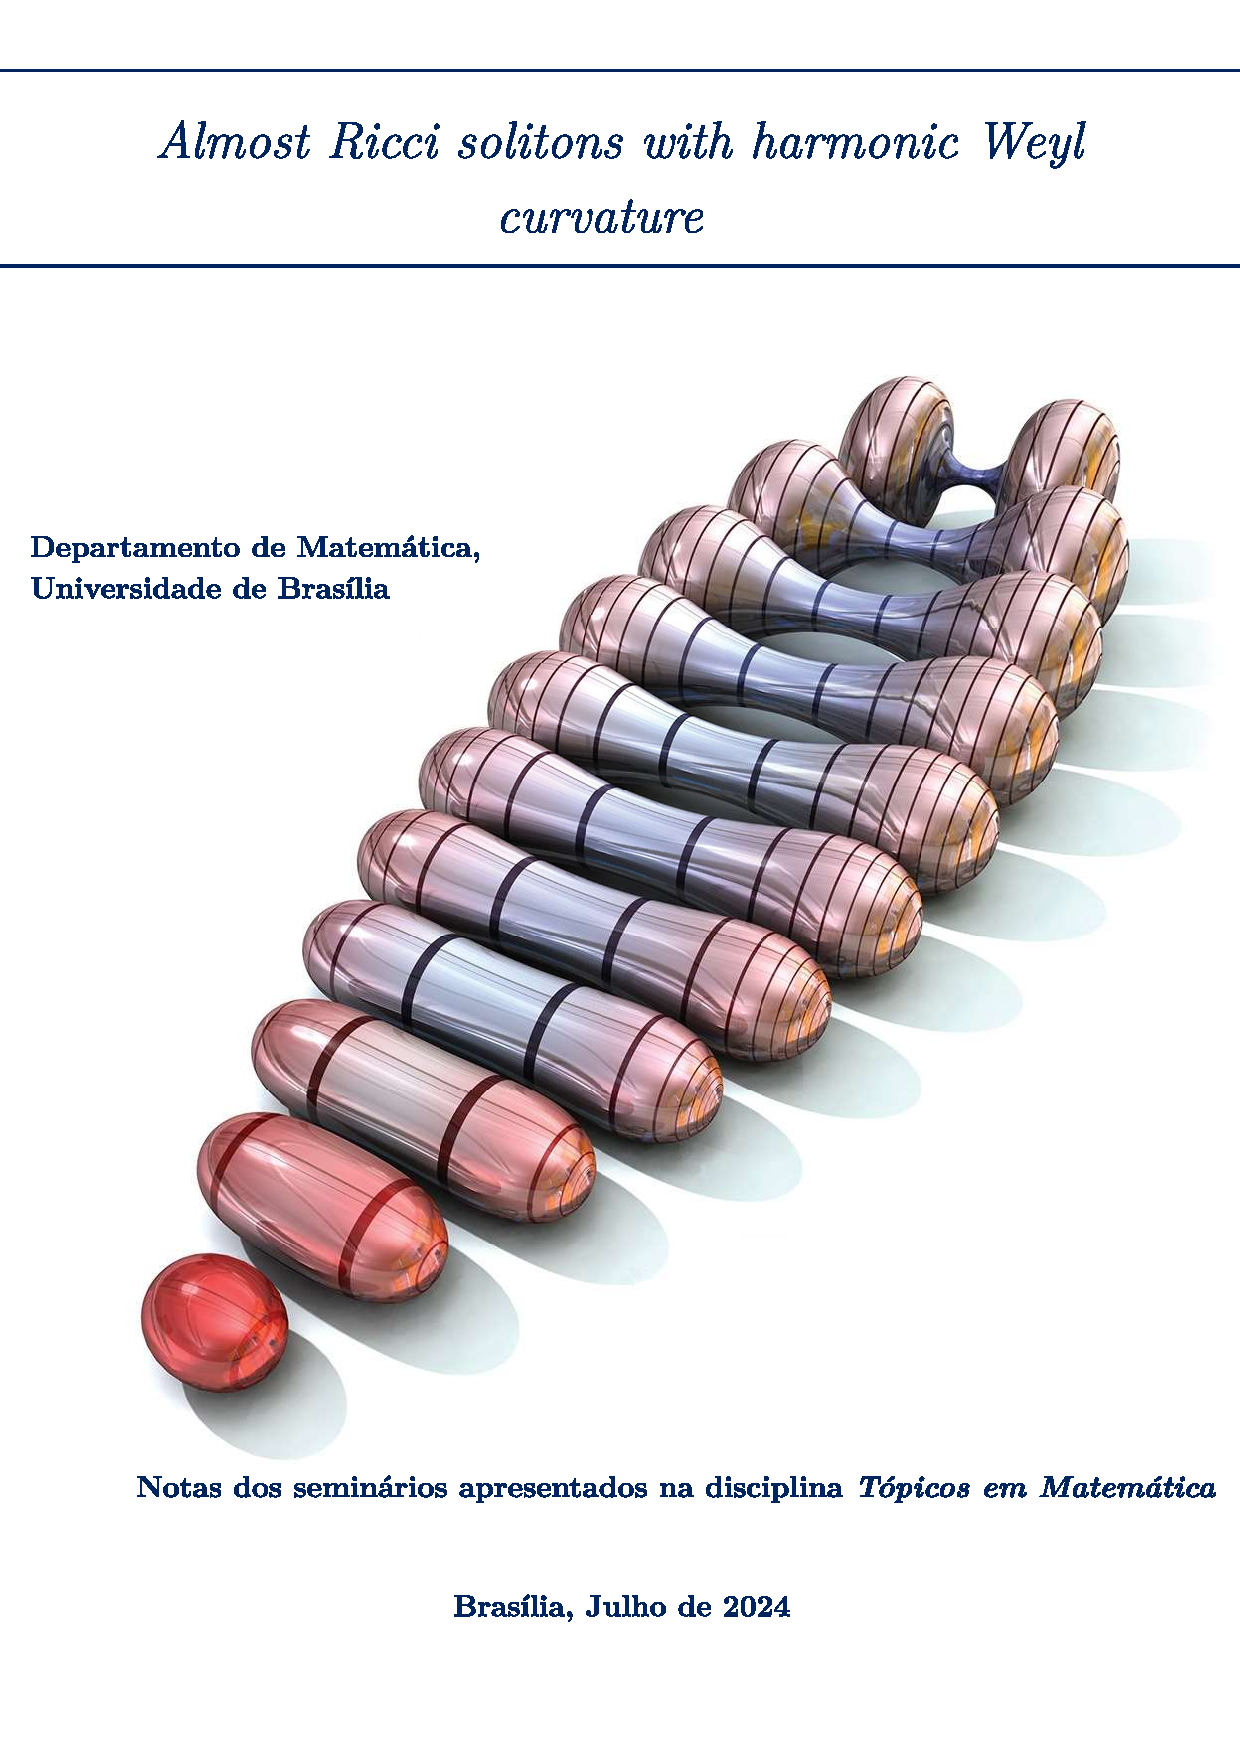
\includepdf[pages=1, pagecommand={}]{capaSeminario.pdf}



% \newcommand{\HRule}{\rule{\linewidth}{0.5mm}} % Defines a new command for the horizontal lines, change thickness here
% \begin{center} % Center everything on the page
 
% %----------------------------------------------------------------------------------------
% %	HEADING SECTIONS
% %----------------------------------------------------------------------------------------


% \PlaceText{15mm}{27mm}{ \color{gal}\noindent\makebox[\linewidth]{\rule{2\paperwidth}{1.5pt}}}

% \PlaceText{67mm}{40mm}{\huge \color{gal} \textit{Almost Ricci Solitons}}

% \PlaceText{51mm}{55mm}{\huge \color{gal} \textit{with harmonic Weyl curvature}}


% \PlaceText{15mm}{62mm}{ \color{gal}\noindent\makebox[\linewidth]{\rule{2\paperwidth}{1.5pt}}}


% \PlaceText{7mm}{20mm}{ 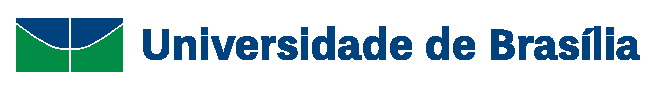
\includegraphics[scale=0.7]{unb.eps}}



% \end{center}

% \vspace{1.5cm}


\pagestyle{fancy}
\renewcommand{\footrulewidth}{0pt}
\fancyhf{}
% \lfoot{\textbf{MATHEUS A. R. M. HORÁCIO | 231107376}}
%\rfoot{\textbf{MATRÍCULA: 17/0110923 }}
\fancyfoot[RO, RE]{\hspace*{2cm} \textbf{Página \thepage \ de \pageref*{LastPage}}}
  \renewcommand\footrule{%

 \color{BlueViolet}\noindent\makebox[\linewidth]{\rule{\paperwidth}{1pt}}
}

\renewcommand{\headrulewidth}{0pt}

        \section{O fluxo de Ricci}
        O fluxo de Ricci surgiu na década de 1980 como a ferramenta mais promissora para a resolução da conjectura de Poincaré. O plano de ataque é o seguinte: tomemos $\mm^3$ uma $3$-variedade topológica fechada simplesmente conexa. Lembrando que em dimensão $n \leq 3$, acontece o seguinte fenômeno muito notável:
\begin{lema}
\textit{Seja $\mm^n$ uma variedade topológica de dimensão $n \leq 3$. Então $\mm^n$ admite uma única estrutura diferenciável compatível com a sua topologia. Consequentemente, 
\[
\mm^n \text{ é homeomorfa a } \mathcal{N}^n  \iff \mm^n \text{ é difeomorfa a }  \mathcal{N}^n 
\]
}
\end{lema}
\begin{demm}
Consulte \mycitep{overflow}.
\end{demm}





Podemos então munir $\mm^3$ de uma estrutura diferenciável e consequentemente de uma métrica Riemanniana, digamos $g_0$ (que, a priori, não sabemos absolutamente nada sobre). Supondo que, milagrosamente, acontecesse que $g_0$ fosse uma métrica de Einstein, o problema estaria acabado: em dimensão $\leq 3$, métricas de Einstein têm curvatura seccional constante. Como uma consequência trivial do teorema de Cartan-Hadamard, tal curvatura necessariamente seria positiva, e portanto, teríamos a certeza (pelo teorema de Killing-Hopf) que $\mm^3$ é isométrica (em particular, homeomorfa) a $\mathbb{S}^3$.\par 
O plano de ataque desenvolvido por R. Hamilton tenta encontrar tal métrica milagrosa ao deformar $g_0$. De modo grosseiro, pensaremos na variedade como se fosse feita de metal, cuja temperatura varia entre regiões distintas, e iremos deformar a métrica de tal forma que façamos a curvatura fluir de áreas mais curvadas para área menos curvadas, assim como o calor flui de regiões mais quentes a mais frias.
Isso equivale a mudar as métricas do espaço de forma que as distâncias diminuam mais rapidamente nas direções ao longo das quais a curvatura é maior. O melhor cenário possível (que, infelizmente não acontece em geral) é que tal processo eventualmente nos forneça uma métrica final (conceito este que precisa ser formalizado) $g_{\infty}$ que seja de Einstein.\par 
Apesar da \emph{prima facie} plausibilidade e simplicidade de tal plano, há vários detalhes que precisam ser estudados com cuidado. Primeiramente, em dimensão $\geq 3$ temperatura é um objeto muito mais simples que curvatura: enquanto que a temperatura na variedade pode ser pensada como uma função real (que, obviamente, associa a cada ponto sua temperatura), a curvatura, em contraste, é uma função $K : \mathrm{Gr}_2(\mm) \to \mathbb{R}$, que associa um valor a cada direção planar passando por um ponto. Em cada ponto de $\mm$ são necessários \text{seis} números diferentes para descrever $K$. Ao buscarmos um análogo da equação do calor
\[
\frac{\partial}{\partial t} u = \Delta u
\] para a curvatura, precisaremos então combinar todos os números que descrevem a curvatura em alguma qunatidade geométrica que faça sentido independentemente de qualquer escolha de coordenadas e impor alguma fórmula que descreva a sua mudança. \par 
Há essencialmente só uma maneira de prosseguir. O laplaciano é, a grosso modo, um operador que faz médias ao longo de pequenas esferas centradas em torno de um ponto, e, analogamente, o tensor de Ricci é obtido do tensor de curvatura Riemanniano ao fazer a média de curvaturas em diferentes direções. Seja então $\{g(t) \}_{t \in I}$ uma família suave de métricas Riemannianas em $\mm$. Assim motivados, fixemos arbitrariamente $X, Y \in \Gamma(T \mm)$ e $p \in \mm$. Para cada $t_0 \in I$ arbitrariamente fixado, o objeto geométrico $\Ric_{g(t_0)}$ está bem definido, a correspondência $(Z, W) \mapsto \Ric_{g(t_0)}(Z, W)$ é um $2$-tensor simétrico e $\Ric_{g(t)}(p)(X(p), Y(p))\in \mathbb{R}$. 
Analogamente, temos $g(t_0)(p)(X(p), Y(p)) \in \mathbb{R}$. Podemos portanto tomar derivadas: vemos que $\frac{\partial}{\partial t}\left(g(t)(X(p), Y(p)) \right) \in \mathbb{R}$, e a correspondência $(Z, W) \mapsto \frac{\partial}{\partial t} \left(g(t)(X, Y) \right)$ é um tensor simétrico. Em particular, fixando uma constante $c \in \mathbb{R}$, a equação
\[
\frac{\partial}{\partial t} g(t) = c \cdot \Ric_{g(t)}
\]
faz sentido. Em vista do seguinte
\begin{lema}
\textit{Em coordenadas harmônicas com respeito a $g(t)$, o tensor de Ricci satisfaz
\begin{equation}\label{calRicci}
c \cdot \Ric_{jk} = -\frac{c}{2} \cdot \Delta(g_{jk}) - \frac{c}{2} \cdot Q_{jk}(\partial g, g^{-1})
\end{equation}
onde $Q_{jk}$ denota uma soma de termos que contém componentes de $g^{-1}$, e derivadas espaciais de ordem $\leq 1$ dos componentes da métrica $g$.
}
\end{lema}
\begin{demm}
    Consulte \mycitep{Adam}, onde \cref{calRicci} foi (equivalentemente) demonstrada no caso $c = -2$.
\end{demm}

\begin{oobs}
    No caso $c = 1$, é comum encontrar na literatura a equação acima escrita como
    \[
    \Ric_{ij} = -\frac{1}{2} \Delta g_{ij} + \text{ termos de ordem } \leq 1
    \]
    \end{oobs}
    É natural então escolher $c = -2$, de forma que, informalmente, a equação do fluxo se escreva como
    \[
    \partial_t g = \Delta g + \cdots
    \] 
    cumprindo o nosso objetivo de encontrar um análogo da equação do calor para a curvatura e justificando a seguinte
    \begin{deff}
      \textit{
      Seja $(\mm, g_{\mm})$ uma variedade Riemanniana e $T > 0$. Diremos que uma família de métricas $\{g_t\}_{t \in [0, T)}$ é uma solução do fluxo de Ricci em $\mm$ com condição inicial $g_{\mm}$ quando
      \begin{equation}\label{eqFluxoRicci}
      \begin{cases}
      \frac{\partial g_t}{\partial t} = - 2 \cdot \Ric_{g_t}, \ \forall t \in (0, T) \\
      g_0 = g_{\mm}
      \end{cases}
      \end{equation}
      }
      \end{deff}
      \begin{oobs}\label{provaPerelman}
        Apesar do plano de ataque acima ter sido inicialmente elaborado para atacar a conjectura de Poincaré, Perelman o estendeu de forma a atacar o problema ainda mais geral da conjectura da geometrização de Thurston. Um dos vários obstáculos nesse sentido é a existência de possíveis singularidades ao longo da evolução do fluxo. Inicialmente, para contornar esse impasse, Hamilton propôs fazer \quotes{cortes} (formalmente, decompor a variedade em somas conexas) na variedade e então reiniciar o fluxo em cada pedaço. Tal processo é comumente chamado de \emph{cirurgia}. \par 
        Idealmente, se espera que somente um número finito de cirurgias tenha de ser realizado e que o fluxo forneça em cada componente uma métrica modelada por uma das oito geometrias-modelo de Thurston, de forma que ao \quotes{voltarmos no tempo}, fazendo a cirurgia no sentido contrário, estejam provadas tanto a conjectura da geometrização de Thurston quanto a conjectura de Poincaré (no caso em que a variedade inicial é simplesmente conexa, se espera que cada componente da cirurgia seja uma esfera - como somas conexas de esferas são esferas, provaríamos a conjectura de Poincaré). \par 
        \begin{figure}[H]
        \centering
        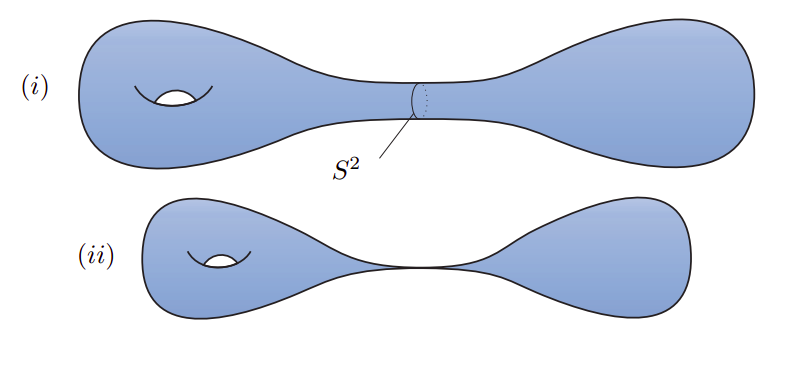
\includegraphics[scale=.5]{nneck.png}
        \vspace{-1cm}
        \caption{uma singularidade do tipo \quotes{pescoço pinçado}. Figura extraída de \mycitep{topping}.}
        \end{figure}
        \begin{figure}[H]
        \centering
        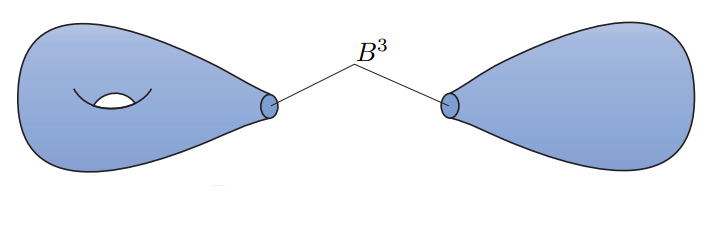
\includegraphics[scale=.5]{ccirurgia.png}
        \caption{cirurgia. Figura extraída de \mycitep{topping}.}
        \end{figure}
        Hamilton não conseguiu mostrar que tal processo não ficava preso numa situação do tipo do paradoxo de Zeno. \emph{A priori}, poderia acontecer que após $1$ segundo de evolução do fluxo tivéssemos que realizar tal processo pela primeira vez (gerando $2$ componentes), após mais $\frac{1}{2}$ segundo tivéssemos que realizá-lo pela segunda vez (gerando $4$ componenentes), após mais $\frac{1}{4}$ de segundo, pela terceira vez (gerando $8$ componentes), e assim sucessivamente... Perelman mostrou que tal obstáculo podia de fato ser superado, ou seja, que só um número finito de cirurgias precisa ser realizado. 
        \end{oobs}
        
        \begin{oobs}
        A ideia de Hamilton para classificar as singularidades foi aplicar mudanças de escala a fim de diminuir a curvatura.
        \begin{figure}[H]
        \centering
        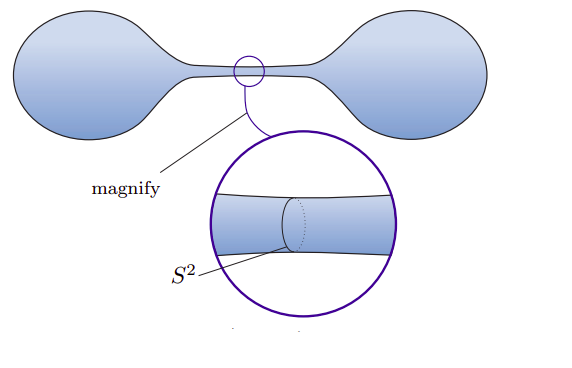
\includegraphics[scale=.4]{blowup.png}
        \vspace{-0.8cm}
        \caption{estratégia para classificar singularidades: usar uma \quotes{lupa} perto da singularidade (aplicar mudanças de escala) com \quotes{zoom} cada vez maior, e então aplicar limites. Figura extraída de \mycitep{topping}.}
        \end{figure}
        Os sólitons de Ricci aparecem como limites do processo que delineamos informalmente na figura acima (cuja formalização pode ser encontrada em \mycitep{HamRicciFlow} ou \mycitep{topping}). Além disso, uma vez que sólitons (que definiremos em breve) são, de certa forma, soluções estacionárias do fluxo, os mesmos \quotes{nascem} como uma grande obstrução inicial ao plano que esboçamos na \cref{provaPerelman}, se tornando assim importantes objetos de estudo.  
        \end{oobs}



  \section{Sólitons de Ricci}
  Uma das obstruções ao programa inicial de Hamilton de evoluir uma métrica Riemanniana inicial arbtirária a uma métrica de curvatura uniforme (em dimensão $3$, Einstein) são os \emph{sólitons de Ricci}. Geometricamente, essas soluções evoluem sob o fluxo apenas por difeomorfismos e mudanças de escala, e são, de certa forma, pontos fixos do fluxo (num sentido a ser formalizado em breve).
  
  \begin{deff}\label{defSoliton}
  Seja $\{g(t)\}_{t \in I}$ uma solução do fluxo de Ricci numa variedade Riemanniana $(\mm, g_0)$. Se existir uma família temporal de difeomorfismos $\{ \varphi_t : \mm \to \mm\}_{t \in I}$ $\left(\text{com $\varphi_0 = \operatorname{Id}_{\mm}$ }\right)$ e um fator de escala temporal $\sigma \in \mathscr{C}^{\infty}(I)$ (com $\sigma(0) = 1$) tal que
  \begin{equation}\label{RicSoliton}
  g(t) = \sigma(t) \cdot \varphi_t^{*}(g_0)
  \end{equation}
  diremos que a solução $\{g(t) \}_{t \in I}$ é um sóliton de Ricci em $\mm$. A tripla $\pa{\{g(t) \}_{t \in I}, \{\varphi_t \}_{t \in I}, \sigma }$ é chamada de \emph{uma estrutura de sóliton de Ricci em $\mm$.}
  \end{deff}
  
  \begin{oobs}
  Denotando por ${\sf Met}(\mm) \doteq \operatorname{Sym}_2^{+}(T^{*}\mm)$ o espaço de métricas Riemannianas em $\mm$, por ${\sf Diff}(\mm)$ o grupo de difeomorfismos de $\mm$ e usando o fato de que o tensor de Ricci é invariante por difeomorfismos, podemos ver o fluxo de Ricci como um sistema dinâmico no espaço 
  \[
  {\sf Met}(\mm) / {\sf Diff}(\mm)
  \] de forma que os sólitons de Ricci correspondem a pontos fixos.
  \end{oobs}


  \begin{proposicao}\label{PropEstrutura}
    Uma variedade Riemanniana $(\mm, g_{\mm} = g_0)$ admite uma estrutura de sóliton de Ricci se, e somente se, existe um campo $V \in \Gamma(T \mm)$ e uma constante $\lambda \in \mathbb{R}$ tal que
    \begin{equation}\label{EqVSoliton}
    \Ric_{g_{\mm}} + \frac{1}{2} \cdot \mathscr{L}_{V} \left( g_{\mm} \right) = \lambda \cdot g_{\mm} 
    \end{equation}
  \end{proposicao}

  \begin{demm}
    Consule \mycitep{MinhaDissertacao}.
  \end{demm}



  \begin{oobs}
    Na literatura, os casos $\lambda > 0$, $\lambda = 0$ e $\lambda < 0$ correspondem a sólitons \emph{shrinking, steady} (\quotes{encolhedores} e \quotes{estáveis/firmes}) e \emph{expanding} (\quotes{expansores}).
    \end{oobs}


    \begin{oobs}\label{OGradSoliton}
      Usando a notação da proposição \cref{PropEstrutura}, diremos que um sóliton de Ricci é um sóliton de Ricci gradiente se existir $f \in \mathscr{C}^{\infty}(\mm)$ tal que $V = \nabla f$. Nesse caso, a equação \cref{EqVSoliton} se escreve como
      \begin{equation}\label{GradSoliton}
      \Ric + \nabla^2 f = \lambda g
      \end{equation}
      Motivados por tal equação, temos também a seguinte
      \end{oobs}
      

\section{Almost Ricci solitons with harmonic Weyl curvature}
      Nessa seção faremos uma classificação local de quase-sólitons de Ricci gradiente com curvatura de Weyl harmônica. Esse é um trabalho em conjunto com Valter Borges Sampaio Junior e João Paulo dos Santos.
      \begin{deff}\label{DefAlmostGradSoliton}
      A Riemannian manifold $\pa{\mm, g}$ is called a gradient almost Ricci soliton  if there exist smooth $f, \lambda \in \mathscr{C}^{\infty}(\mm)$ such that 
      \begin{equation}\label{AlmostGradSoliton}
      \Ric + \nabla^2 f = \lambda g
      \end{equation}
      \end{deff}

      \begin{oobs}
        Assim como sólitons de Ricci evoluem somente por mudanças de escalas e difeomorfismos, quase-sólitons de Ricci evoluem somente por difeomorfismos conformes. Para detalhes, veja \mycitep{DifConf1} e \mycitep{DifConf2}.
        \end{oobs}

        Our main results are the following:
        

        \begin{teorema}\label{decompwarp-INTRO}
            Any gradient almost Ricci soliton with harmonic Weyl curvature is a multiply warped product metric.
            \end{teorema}

            We shall see that the fibers of this warped product are, in fact, the integrable submanifolds of the distributions corresponding to the eigenspaces of the Ricci tensor.

            \begin{teorema}\label{maxxnumeig-INTRO}
                Let $(\mm^n,g,f,\lambda)$ be a gradient almost Ricci soliton, not necessarily complete, with harmonic Weyl curvature, nonconstant $f$ and $n\geq4$. Then its Ricci tensor has at most three distinct eigenvalues at each point.
            \end{teorema}

            Theorem \cref{maxxnumeig-INTRO} generalizes Kim's result from \mycitep{kim2}, which was proven only for $n = 4$.


            \begin{teorema}[Local warped product structure]\label{T31-INTRO}
                Let $\pa{\mm^n, g, f, \lambda}$ be an almost Ricci soliton with $n \geq 4$ and $f$ non constant. Assume the soliton has harmonic Weyl curvature and that its Ricci tensor has exactly two distinct eigenvalues. Then for any point $p\in\mathcal{R}\cap \mm_{\mathcal{A}}$ there are a neighborhood $U\subset\mathcal{R}\cap \mm_{\mathcal{A}}$ of $p$ and a warped product $I \times_{h} \nn$ of an interval and an Einstein manifold $\nn^{n-1}$ so that $U$ is isometric to a domain of $I \times_{h} \nn$. Furthermore, $f$ and $\lambda$ are constant on $\nn$, through the identification between $I \times \nn$ and $U$.
           \end{teorema}
           
           Theorem \cref{T31-INTRO} allows us to construct examples of gradient almost Ricci solitons for any given warping function $h$. 
           
           
           \begin{teorema}[Local multiply warped product structure]\label{localstrucDuplo-INTRO}
               Let $\pa{\mm^n, g, f, \lambda}$ be an almost Ricci soliton with $n \geq 4$ and $f$ non constant. Assume the soliton has harmonic weyl curvature and that its Ricci tensor has exactly three distinct eigenvalues. Then for any point $p\in\mathcal{R}\cap \mm_{\mathcal{A}}$ there are a neighborhood $U\subset\mathcal{R}\cap \mm_{\mathcal{A}}$ of $p$ and a multiply warped product $I \times_{h_1} \nn_1 \times_{h_2} \nn_2$ of an interval $I$ and two Einstein manifolds $\nn_1$ and $\nn_2$, so that $(U,g)$ is isometric to a domain of $I \times_{h_1} \nn_1 \times_{h_2} \nn_2$. Furthermore, $f$ and $\lambda$ are constant on $\nn_{1}\times\nn_{2}$, through the identification between $I\times\nn_{1}\times\nn_{2}$ and $U$.
               \end{teorema}


               \subsection{Preliminaries}
Along this work we will adopt the following convention for the curvature
\begin{align}
	\Rm(X,Y,Z,W)=\left\langle\nabla_{Y}\nabla_{X}Z-\nabla_{X}\nabla_{Y}Z+\nabla_{[X,Y]}Z,W\right\rangle,
\end{align}
for vector fields $X,Y,Z,W\in\mathfrak{X}(M)$. When $\mm$ is an Einstein manifold, we will denote its Einstein constant (i.e. the constant value $\Ric_{\mm}$ takes on the unit tangent bundle of $\mm$) by $\lambda_{\mm}$. Similarly, its constant scalar curvature (equal to $\dim(\mm) \lambda_{\mm}$) will be denoted by $\tau_{\mm}$.


\begin{lema}[Barros-Ribeiro]\label{bari}
	A gradient almost Ricci soliton $(\mm^n,g,f,\lambda)$ has harmonic Weyl curvature if, and only if,
	\begin{align*}
		\Rm(\nabla f,X,Y,Z)&=Y\left(\frac{R}{2(n-1)}-\lambda\right)g(X,Z)-Z\left(\frac{R}{2(n-1)}-\lambda\right)g(X,Y)\nonumber\\
		&=\frac{1}{n-1}(\Ric(\nabla f,Y)g(X,Z)-\Ric(\nabla f,Y)g(X,Y))
	\end{align*}
\end{lema}


\begin{lema}[Cao-Chen]\label{caochen}
	Let $(\mm,g,f,\lambda)$ be a gradient almost Ricci soliton with harmonic Weyl curvature and non-constant $f$. Let $c$ be a regular value of $f$ and $\Sigma_{c}=f^{-1}(c)$ be the level surface of $f$. Then,
	\begin{enumerate}
		\item Where $\nabla f\neq0$, $E_{1}=\frac{\nabla f}{|\nabla f|}$ is an eigenvector of $\Ric$.
		\item $|\nabla f|$ is constant on a connected component of $\Sigma_{c}$.
		\item There is a function $s$ locally defined with $s(x)=\int\frac{\dd f}{|\nabla f|}$, so that $\dd s=\frac{\dd f}{|\nabla f|}$ and $E_{1}=\nabla s$.
		\item\label{cao4} $E_{1}E_{1}f=-\Ric(E_{1},E_{1})+\lambda$. In particular, $-\Ric(E_{1},E_{1})+\lambda$ is constant on a connected component of $\Sigma_{c}$.
		\item Near a point in $\Sigma_{c}$, the metric $g$ can be written as
		\[
			g=\dd s^2+\sum_{i,j\geq2}g_{ij}(s,x_{2},\ldots,x_{n}) \ \dd x_{i}\otimes \dd x_{j}.
		\]
		\item $\nabla_{E_{1}}E_{1}=0$.
	\end{enumerate}
\end{lema}

It is a well known fact that a Riemannian manifold $(M^{n},g)$, $n\geq4$, has harmonic Weyl tensor if and only if its Schouten tensor $\mathcal{A}=\Ric-\frac{R}{2(n-1)}g$ is Codazzi. In coordinates this is equivalent to
\begin{align}
	\nabla_{i}\mathcal{A}_{jk}=\nabla_{j}\mathcal{A}_{ik}.
\end{align}
Let $\mathcal{A}$ be a codazzi tensor and denote by $E_{\mathcal{A}}(x)$ the number of distinct eigenvalues of $\mathcal{A}$ at $x$. In \cite{derd}, Derdzinski considered the following open dense set
\begin{align}
	\mm_{\mathcal{A}}=\{x\in \mm \ |  \ E_{\mathcal{A}}(x)\text{ is constant in a neighborhood of }x\}.
\end{align}
It turns out that in $\mm_{\mathcal{A}}$ the eigenvalues of $\mathcal{A}$ are well defined and define smooth functions $\lambda_{1},\ldots,\lambda_{n}:\mm_{\mathcal{A}}\rightarrow\mathbb{R}$. Furthermore, he proved that in such a set the following is true
%{\color{red}Enunciar o lema abaixo pra campos gerais nas auto-dstribuições.}
\begin{lema}[Derdzi\'{n}ski]\label{derdlema}
	Let $(\mm^n,g)$, $n\geq4$, be a Riemannian metric with harmonic Weyl curvature. Let $\{E_{i}\}_{i=1}^{n}$ be a local orthonormal frame such that $\Ric(E_{i},\cdot)=\lambda_{i}g(E_{i},\cdot)$. Then,
	\begin{enumerate}
		\item\label{derd1} For any $i,j,k\geq1$,
		\begin{align*}
		(\lambda_{j}-\lambda_{k})\left\langle\nabla_{E_{i}}E_{j},E_{k}\right\rangle+\nabla_{E_{i}}(\mathcal{A}(E_{j},E_{k}))=\\
		(\lambda_{i}-\lambda_{k})\left\langle\nabla_{E_{j}}E_{i},E_{k}\right\rangle+\nabla_{E_{j}}(\mathcal{A}(E_{k},E_{i})).
		\end{align*}
		\item If $k\neq i$ and $k\neq j$, then $(\lambda_{j}-\lambda_{k})\left\langle\nabla_{E_{i}}E_{j},E_{k}\right\rangle=(\lambda_{i}-\lambda_{k})\left\langle\nabla_{E_{j}}E_{i},E_{k}\right\rangle$.
		\item Given distinct eigenfunctions $\lambda$ and $\mu$ of $\mathcal{A}$ and local vector fields $U$ and $V$ such that $AV=\lambda V$ and $AU=\mu U$ with $|U|=1$, it holds that $V(\mu)=(\mu-\lambda)\left\langle\nabla_{U}U,V\right\rangle$.
		\item Each distribution $D_{\lambda_{i}}$, defined by $D_{\lambda_{i}}(p)=\{v\in T_{p} \mm \ | \ \Ric(v,\cdot)=\lambda_{i}g(v,\cdot)\}$, is integrable	 and its leaves are totally umbilic submanifolds of $M$.
	\end{enumerate}
\end{lema}


\subsection{Local structure}

Suppose that the potential function of the almost soliton $\mm$ is nonconstant and consider the set $\mathcal{R}$ of all regular points of $f$
\begin{align*}
	\mathcal{R}=\{x\in \mm \ | \ \nabla f(x)\neq0\}.
\end{align*}

We start with the following result.
\begin{lema}\label{denseempty}
	Let $(\mm^{n},g,f,\lambda)$ be a gradient almost Ricci soliton with harmonic Weyl curvature. If $f$ is not constant and $W$ is a connected component of $\mm_{\mathcal{A}}$, then either $W\cap\mathcal{R}$ is dense in $W$, or it is empty.
\end{lema}
% \begin{demm}
% 	Let $W$ be a connected component of $M_{\mathcal{A}}$ so that $W'=W\cap\mathcal{R}\neq\emptyset$. We will show that $W'$ is dense in $W$. Suppose by contradiction that  this is not true and consider an open set $U\subset W\backslash W'$. Once $\nabla f$ vanishes in $U$, the almost Ricci soliton equation becomes $\Ric=\lambda g$ in $U$. As the quantity of eigenvalues of $\Ric$ is constant in $W$, it follows that $\mm$ is Einstein in this set, i.e., there is $\mu\in\mathbb{R}$ so that $\Ric=\mu g$ in $W$. In particular, $\nabla\nabla f=(\lambda-\mu)g$ in $W$. Using the Bochner formula we obtain
% 	\begin{align*}
% 		X(\lambda)=\operatorname{div}(\nabla\nabla f)(X)=\Ric(\nabla f,X)+X(\Delta f)=X(\mu f+n\lambda),\ \forall X\in\mathfrak{X}(W),
% 	\end{align*}
% 	which implies the existence of $c_{0}\in\mathbb{R}$ so that $\displaystyle\lambda=-\frac{\mu}{n-1}f+\mu+c_{0}$. Consequently,
% 	\begin{align*}
% 		\nabla\nabla f=\left(-\frac{\mu}{n-1}f+c_{0}\right)g,\ \text{in}\ W.
% 	\end{align*}
% 	Now observe that if $\mu\neq0$, then $\displaystyle f-\frac{(n-1)c_{0}}{\mu}$ is an eigenfunction of $-\Delta$. If, on the other hand, $\mu=0$, then $\lambda$ is constant, $\Ric=0$ and $\nabla\nabla f=\lambda g$, which means that $(W,g|_{W},f,\lambda)$ is a Ricci soliton. In both cases we conclude that $f$ is analytic in $W$. As $\nabla f$ vanishes in $U$, $f$ is constant in $W$, contradicting our assumption.
	
% 	This means that $W\backslash W'$ has empty interior or, equivalently, that the set $W'$ is dense in $W$.
% %	Along this proof we only consider the topology relative to $M_{\mathcal{A}}$. Suppose by contradiction that $\mathcal{S}=M_{\mathcal{A}}-\mathcal{R}$ has nonempty interior and let $p_{0}$ be a point in the boundary of the interior of $\mathcal{S}$ (contained in $M_{\mathcal{A}}$). Recall that any point in $M_{\mathcal{A}}$ has an open neighborhood in which the number of distinct eigenvalues of $Ric$ is constant and denote by $U$ one of these neighborhoods containing $p_{0}$. Observe that in the interior of $\mathcal{S}$ the almost Ricci soliton equation yields $Ric=\lambda g$. Consequently, the same holds in $U$. As each point in the boundary of $U$ which is contained in $M_{\mathcal{A}}$ has a neighborhood in which $Ric$ has a constant number of eigenvalues, we prove that $Ric=\lambda g$ all over $M_{\mathcal{A}}$. In particular, $\lambda$ is constant and $f$ is analytic. Once there is an open subset in $\mathcal{S}$, analyticity implies the constancy of $f$, which is a contradiction.
% \end{demm}

For each point $p$ of the open set $\mathcal{R}\cap M_{\mathcal{A}}$, we will consider the orthonormal frame $\{E_{i}\}_{i=1}^n$ given in lema \ref{derdlema} and recall that $E_{1}=\frac{\nabla f}{|\nabla f|}$. For this frame, we have $R_{ij}=\lambda_{i}\delta_{ij}$. Furthermore,
\begin{lema}\label{nablaframe}
	Let $(\mm^n,g,f,\lambda)$, $n\geq4$, be a gradient almost Ricci soliton with harmonic Weyl curvature and nonconstant $f$. Then,
	\begin{align}\label{step2}
		 \nabla_{E_{a}}E_{1}=\xi_{a}E_{a}\ \ \text{and}\ \ \xi_{a}=-\left\langle\nabla_{E_{a}}E_{a},E_{1}\right\rangle,
		%\item $\nabla_{E_{1}}E_{a}=\displaystyle\sum_{c\in[a]}A_{1a}^{c}E_{c}$ and $\nabla_{E_{b}}E_{a}=\displaystyle\sum_{c\in[a]}A_{ab}^{c}E_{c}$.
	\end{align}
	where
	\begin{align}\label{step1}
		\xi_{a}=\frac{\lambda-\lambda_{a}}{|\nabla f|}.
	\end{align}
\end{lema}
\begin{demm}
To prove the first identity of $(\ref{step2})$, notice that for any $a\geq2$ we have
\begin{align}\label{comp1}
	\begin{split}
	\nabla_{E_{a}}E_{1}=\frac{\nabla_{E_{a}}\nabla f}{|\nabla f|}=\frac{\lambda E_{a}-\Ric(E_{a},\cdot)}{|\nabla f|}=\frac{(\lambda-\lambda_{a})E_{a}}{|\nabla f|}=\xi_{a}E_{a}.
	\end{split}
\end{align}
Now we combine it with the equality $\left\langle\nabla_{E_{a}}E_{1},E_{a}\right\rangle=-\left\langle\nabla_{E_{a}}E_{a},E_{1}\right\rangle$ to get the second identity of $(\ref{step2})$. \\

\end{demm}



The next lemma is a generalization to nonconstant $\lambda$ of Lemma 3.3 from \mycitep{feng}, which is already an extension of lemma 2.7 from \mycitep{kim1} to higher dimensions of its counterpart for four dimensional Ricci solitons.
\begin{lema}
	Let $(\mm^n,g,f,\lambda)$, $n\geq4$, be a gradient almost Ricci soliton with harmonic Weyl curvature and nonconstant $f$. The functions $\lambda_{2},\ldots,\lambda_{n}$ are constant on each connected component of $\Sigma_{c}$. As a consequence, the functions $\xi_{2},\ldots,\xi_{n}$ are also constant on each connected component of $\Sigma_{c}$.
\end{lema}




Following \mycitep{feng}, for each $a\geq2$ we consider the following notation
\begin{align}
	[a]=\{i\in\{2,\ldots,n\} \ | \ \lambda_{i}=\lambda_{a}\}.
\end{align}
From now on we use the convention that $2\leq a,b,c,\ldots,\alpha,\beta,\gamma,\ldots\leq n$ satisfy $b,c\in[a]$, $\beta,\gamma\in[\alpha]$ and $[a]\neq[\alpha]$.

\begin{lema}\label{lemmamany}
	Let $(\mm^n,g,f,\lambda)$, $n\geq4$, be a gradient almost Ricci soliton with harmonic Weyl curvature and nonconstant $f$. Let $(x_{b})_{b\in[a]}$ and $(x_{\beta})_{\beta\in[\alpha]}$ be local coordinate systems of the integral manifolds of the distributions $D_{a}$ and $D_{\alpha}$, respectively . Setting $\partial_{1}=E_{1}$, we have
	\begin{enumerate}
		\item\label{1} $\nabla_{\partial_{a}}{\partial_{1}}=\xi_{a}\partial_{a}$ and $\nabla_{\partial_{a}}\partial_{b}=-\xi_{a}g_{ab}\partial_{1}+\displaystyle\sum_{c\in[a], c\neq a}\Gamma_{ab}^{c}\partial_{c}$.
		%\item\label{2} $\nabla_{\partial_{1}}\partial_{a}=\displaystyle\sum_{c\in[a]}\Gamma_{1a}^{c}\partial_{c}$ and $\nabla_{\partial_{b}}\partial_{a}=\displaystyle\sum_{c\in[a]}\Gamma_{ab}^{c}\partial_{c}$.
		\item\label{3} $\nabla_{\partial_{\alpha}}\partial_{a}=0$.
		\item\label{4} $R_{1a1b}=-(\xi_{a}'+\xi_{a}^{2})g_{ab}$.
		\item\label{5} $R_{a\alpha b\beta}=-\xi_{a}\xi_{\alpha}g_{ab}g_{\alpha\beta}$
	\end{enumerate}
	In particular,
	\begin{align}\label{37lemma36}
		 \partial_{1}g_{ab}=2\xi_{a}g_{ab}\ \ \ \ \text{and}\ \ \ \ \ \partial_\alpha g_{ab}=0.
	\end{align}
\end{lema}
\begin{demm}
	Proceeding as in $(\ref{comp1})$, for any vector field $X$ and any $a\geq2$ we have
	\begin{align*}
		\left\langle\nabla_{\partial_a}\partial_{1},X\right\rangle=\frac{1}{|\nabla f|}\nabla\nabla f(\partial_a,X)=\frac{\lambda-\lambda_{a}}{|\nabla f|}\left\langle\partial_{a},X\right\rangle=\left\langle\xi_{a}\partial_{a},X\right\rangle,
	\end{align*}
	which proves the first equality of $(\ref{1})$. The second one follows from $g_{1a}=0$ and from
	\begin{align*}
		\left\langle\nabla_{\partial_a}\partial_{b},\partial_{1}\right\rangle=-\left\langle\nabla_{\partial_a}\partial_{1},\partial_{b}\right\rangle=-\xi_{a}g_{ab}.
	\end{align*}

	Now we proceed to prove $(\ref{3})$. If $a,\alpha,z\in\{2,\ldots,n\}$ are so that $[a]\neq[\alpha]$, then
	\begin{align*}
		R_{a\alpha1z}&=\left\langle\nabla_{\partial_{\alpha}}\nabla_{\partial_{a}}\partial_{1}-\nabla_{\partial_{a}}\nabla_{\partial_{\alpha}}\partial_{1},\partial_{z}\right\rangle\\
		&=\xi_{a}\left\langle\nabla_{\partial_{\alpha}}\partial_{a},\partial_{z}\right\rangle-\xi_{\alpha}\left\langle\nabla_{\partial_{a}}\partial_{\alpha},\partial_{z}\right\rangle\\
		&=(\xi_{a}-\xi_{\alpha})\left\langle\nabla_{\partial_{\alpha}}\partial_{a},\partial_{z}\right\rangle.
	\end{align*}
	On the other hand, by using $(\ref{bari})$ we obtain
	\begin{align*}
		(\xi_{a}-\xi_{\alpha})\left\langle\nabla_{\partial_{\alpha}}\partial_{a},\partial_{z}\right\rangle&=R_{1za\alpha}\\
		&=\partial_{a}\left(\frac{R}{2(n-1)}-\lambda\right)g_{z\alpha}-\partial_{\alpha}\left(\frac{R}{2(n-1)}-\lambda\right)g_{za}\\
		&=0,
	\end{align*}
	where in the last line we have used that $\partial_{i}\lambda=\partial_{i}R=0$ for all $i\geq2$. As $[a]\neq[\alpha]$ and $z\in\{1,\ldots,n\}$, we conclude that $\nabla_{\partial_{\alpha}}\partial_{a}=0$.
	
	Using $(\ref{1})$ and $(\ref{3})$ we get
	\begin{align*}
		R_{1a1b}&=\left\langle\nabla_{\partial_{a}}\nabla_{\partial_{1}}\partial_{1}-\nabla_{\partial_{1}}\nabla_{\partial_{a}}\partial_{1},\partial_{b}\right\rangle\\
		%&=-\left\langle\nabla_{\partial_{1}}(\xi_{a}\partial_{a}),\partial_{b}\right\rangle\\
		&=-\left\langle\xi_{a}'\partial_{a}+\xi_{a}\nabla_{\partial_{1}}\partial_{a},\partial_{b}\right\rangle\\
		%&=-\left\langle\xi_{a}'\partial_{a}+\xi_{a}^2\partial_{a},\partial_{b}\right\rangle\\
		&=-(\xi_{a}'+\xi_{a}^2)g_{ab},
	\end{align*}
	and
	\begin{align*}
		R_{a\alpha b\beta}&=\left\langle\nabla_{\partial_{\alpha}}\nabla_{\partial_{a}}\partial_{b}-\nabla_{\partial_{a}}\nabla_{\partial_{\alpha}}\partial_{b},\partial_{\beta}\right\rangle\\
		&=\displaystyle\left\langle\nabla_{\partial_{\alpha}}\left(-\xi_{a}g_{ab}\partial_{1}+\sum_{c\in[a], c\neq a}\Gamma_{ab}^{c}\partial_{c}\right),\partial_{\beta}\right\rangle\\
		&=\displaystyle-\xi_{a}g_{ab}\left\langle\nabla_{\partial_{\alpha}}\partial_{1},\partial_{\beta}\right\rangle+\sum_{c\in[a], c\neq a}\left\langle\nabla_{\partial_{\alpha}}\left(\Gamma_{ab}^{c}\partial_{c}\right),\partial_{\beta}\right\rangle\\
		&=\displaystyle-\xi_{a}\xi_{\alpha}g_{ab}g_{\alpha\beta}+\sum_{c\in[a], c\neq a}(\Gamma_{ab}^{c}\left\langle\nabla_{\partial_{\alpha}}\partial_{c},\partial_{\beta}\right\rangle+\partial_{\alpha}\Gamma_{ab}^{c}\left\langle\partial_{c},\partial_{\beta}\right\rangle)\\
		&=\displaystyle-\xi_{a}\xi_{\alpha}g_{ab}g_{\alpha\beta},
	\end{align*}
	proving $(\ref{4})$ and $(\ref{5})$, respectively.
	
	In order to finish the proof of the lemma, recall that $\xi_{a}=\xi_{b}$ and consider the following derivatives of $g_{ab}$
	\begin{align*}
		\partial_{1}g_{ab}&=g(\nabla_{\partial_{1}}\partial_{a},\partial_{b})+g(\partial_{a},\nabla_{\partial_{1}}\partial_{b})=2\xi_{a}g_{ab}\\
		\partial_{\alpha}g_{ab}&=g(\nabla_{\partial_{\alpha}}\partial_{a},\partial_{b})+g(\partial_{a},\nabla_{\partial_{\alpha}}\partial_{b})=0.
	\end{align*}
\end{demm}


\begin{teorema}\label{decompwarp}
    Any gradient almost Ricci soliton with harmonic Weyl curvature is a multiply warped product metric of eigenspaces with the Ricci tensor.
    \end{teorema}
    
    \begin{demm}
    Let $U \subset \mathcal{M}_A \cap \{ \nabla f \neq 0 \}$ be an open subset. We'll take local coordinates $(x_1 = s, x_2, x_3, \ldots, x_n)$ in $U$ as in lemma \ref{caochen}. Let us fix $s_0 \in I$ and $a, b \in [i]$. Mutatis mutandis, equation (\ref{37lemma36}) from lemma (\ref{lemmamany}) implies that 
    \[
    \partial_1(g_{ab}) = 2 \xi_a g_{ab}
    \]
    Therefore, if we define the function $\tilde{h}_i: I \to \mathbb{R}$ by
    \[
    s \in I \mapsto \tilde{h}_i(s) := \operatorname{exp}\left(\int_{s_0}^s \xi_a(y) \ \mathrm{d} y \right)
    \]
    Then $\tilde{h}_i$ satisfies
    \[
    \partial_1\left(\tilde{h}_i^{-2} g_{ab} \right) = 0
    \]
    so that $\tilde{h}^{-2}_i g_{ab}$ is constant in $s$, i.e, 
    \[
    (\tilde{h}_i(s))^{-2} g_{ab}(s, x_2, \ldots, x_n) = (\tilde{h}_i(s_0))^{-2} g_{ab}(s_0, x_2, \ldots, x_n)
    \]
    or, equivalently,
    \begin{equation}\label{defm}
    g_{ab}(s, x_2, \ldots, x_n) = h(s)^2 g_{ab}(s_0, x_2, \ldots, x_n)
    \end{equation}
    where $h(s) := \frac{h_i(s)}{h_i(s_0)}$. Without any loss of generality, we can assume $h_i(s_0) = 1$. Clearly, (\ref{defm}) defines a Riemannian metric $g_i$ on $N_i$. In an entirely analogous manner, we obtain Riemannian metrics $g_{\alpha}$ on $N_{\alpha}$ for any $\alpha \notin [i]$. This proves that in $U$, $g$ can be written as the following warped product (of possibly $n-1$ fibers):
    \[
    g = \mathrm{d}s^2 + h_i^2 g_i + \sum_{\alpha \notin [i]} h_{\alpha}^2 g_{\alpha}
    \]
    \end{demm}
    
    \begin{oobs}
        As a straightforward consequence of the proof of theorem \cref{decompwarp}, we get 
        \begin{equation}\label{eqXiRelFuncWarp}
            \frac{\lambda - \lambda_i}{f'} = \xi_i = \frac{h_{i}'}{h_i}
        \end{equation}
        This equation will be useful later on.
    \end{oobs}

    \begin{oobs}
        We'll recognize the amount of fibers in a multiply warped product in the same way as \mycitep{GarciaRio}. Namely, warping functions cannot be constant, two different warping functions cannot be multiples of one another and any two fibers with the same warping function are joined in a single fiber. 
        \end{oobs}

        Now we obtain a local description of $M$, which is a consequence of Lemma \ref{lemmamany} and Theorem \cref{maxxnumeig-INTRO}. First, recall the following formulas for the Ricci and scalar curvatures of a multiply warped product:\\

        \begin{lema}\label{warped}
        Let $\mm = B \times_{h_1} \nn_1^{d_1} \times \cdots \times_{h_k} \nn_{k}^{d_k}$ be a Riemannian multiply warped product with metric $g = g_{B} \oplus h_1^2 g_{\nn_1} \oplus \cdots \oplus h_{k}^2 g_{\nn_k}$. Then the scalar curvature of $\mm$ is given by
        \begin{equation}\label{ScalWarped}
        \begin{aligned}
        R = R_{B} &- 2 \sum_{1 \leq i \leq k} d_i \frac{\Delta_B h_i}{h_i} + \sum_{1 \leq i \leq k} \frac{R_{\nn_i}}{h_i^2} - \sum_{1 \leq i \leq k} d_i(d_i - 1) \frac{\| \grad_B h_i \|_B^2}{h_i^2} \\
        &- \sum_{1 \leq i \leq k} \sum_{\substack{1 \leq \ell \leq k \\
        \ell \neq i  \\
        }} d_i d_{\ell} \frac{g_B(\grad_B h_i, \grad_B h_{\ell})}{h_i h_{\ell}}
        \end{aligned}
        \end{equation}
        Also, for any lifted vector fields $X, Y, Z \in \mathcal{L}(B)$, $V \in \mathcal{L}(\nn_i)$ and $W \in \mathcal{L}(\nn_j)$, we have
        \begin{enumerate}[label=\color{MH}\normalfont\textbf{(\theenumi)}]
        \item\label{NablaWarp} \[
        \nabla_X V = \nabla_V X = \frac{X(h_i)}{h_i} V
        \]
        \item\label{RicXY} \[
        \Ric(X, Y) = \Ric_B(X,Y) - \sum_{1 \leq \ell \leq k} \frac{d_{\ell}}{h_{\ell}} \Hess_B(h_{\ell})(X, Y)
        \]
        \item\label{RicXV} \[
        \Ric(X, V) = 0
        \]
        \item\label{RicVWd} \[
        \Ric(V, W) = 0 \text{ if } i \neq j
        \]
        \item\label{RicVWi} \[ \begin{aligned}
        \Ric(V, W) = \Ric_{\nn_i}(V, W) - &\left(\frac{\Delta_B h_i}{h_i} + (d_i - 1) \frac{\| \grad_{B} h_i \|^2}{h_i^2} \right.\\ &+ \left.\sum_{\substack{1 \leq \ell \leq k \\
        \ell \neq i  \\
        }} d_{\ell} \cdot \frac{g_B(\grad_B h_i, \grad_B h_{\ell})}{h_i h_{\ell}} \right) g(V, W), \text{ if } i = j
        \end{aligned}
        \]
        \end{enumerate}
        \end{lema}
        
        Another interesting fact about warped products is the following
        \begin{teorema}\label{HarmImpliesEinstein}
            Suppose that the multiply warped product $\mm = B \times_{h_1} \nn_1^{d_1} \times \cdots \times_{h_k} \nn_{k}^{d_k}$ with metric $g = g_{B} \oplus h_1^2 g_{\nn_1} \oplus \cdots \oplus h_{k}^2 g_{\nn_k}$ has harmonic Weyl curvature. Then each fiber $\left(\nn_i, g_{\nn_i}\right)$ is an Einstein manifold.
        \end{teorema}
        
        \begin{demm}
        Since $\mm$ has harmonic Weyl curvature, we have
        \begin{equation}\label{CotN}
            \left(\nabla_X \Ric\right)(Y, Z) -  \left(\nabla_Y \Ric\right)(X, Z) = \frac{1}{2n-2} \left\{\left(\nabla_X (Rg)\right)(Y, Z) - \left(\nabla_Y (Rg)\right)(X, Z)\right\}
        \end{equation}
            for all vector fields $ X, Y, Z \in \Gamma\left(T \mm\right)$. In particular, if we take an unitary vector field $\widetilde{V} \in \mathcal{L}(\nn_i)$ and a convenient (in a sense we'll clarify soon) $X \in \Gamma(T \mm)$, we get 
            \begin{align*}
                \left(\nabla_X \Ric\right)(V, V) -  \left(\nabla_V \Ric\right)(X, V) &= \varphi_1 X(h_i) \Ric^{\nn_i}(\widetilde{V}, \widetilde{V})\\
                &=\varphi_2
            \end{align*}
            where $\varphi_1 \neq 0, \varphi_2$ are functions depending only on $\bb$ determined by lemma \cref{warped}. Clearly, this implies that
            \[
                \Ric^{\nn_i}(\widetilde{V}, \widetilde{V}) = \frac{\varphi_3}{X(h_i)} 
                \]
            where $\varphi_3$ is a function which depends on $\bb$ only. Since $h$ is not constant we can always choose $X$ in a way that makes the right-hand side of the above equation well defined. This completes the proof.
        \end{demm}	
        
        Combining theorems \cref{decompwarp}, Theorem \cref{maxxnumeig-INTRO} and \cref{HarmImpliesEinstein}, we get \\
        \begin{teorema}
            Suppose a multiply warped product $\mm = B \times_{h_1} \nn_1^{d_1} \times \cdots \times_{h_k} \nn_{k}^{d_k}$ with metric $g = g_{B} \oplus h_1^2 g_{\nn_1} \oplus \cdots \oplus h_{k}^2 g_{\nn_k}$ has harmonic Weyl curvature and also admits a structure of almost Ricci soliton with non constant $f$. Then $k \leq 2$. \\
        \end{teorema}
        
        \begin{demm}
            This is a straighforward consequence of the equation
            \[
        \lambda_{\alpha} - \lambda_{\beta} = f' \left(\frac{h_{\alpha}'}{h_{\alpha}}  - \frac{h_{\beta}'}{h_{\beta}} \right)
        \] 
        \end{demm}
        
        When there is only a single fiber to be considered, the reciprocal of Theorem \cref{HarmImpliesEinstein} is the following:
        
        \begin{teorema}\label{harmWarp}
            Let $\mm = \mathcal{I} \times_{h} \nn^{n-1}$ be a warped product over an Einstein manifold $\nn$. Then $\mm$ has harmonic Weyl curvature.
        \end{teorema}
        
        \begin{demm}
            Let $\{ \widetilde{E}_i \}_{1 \leq i \leq n}$ be a $g_{\nn}$-orthonormal frame and consider the $g$-orthonormal frame $$\left\{ E_i \doteq \frac{\widetilde{E_i}}{h}\right\}_{1 \leq i \leq n}$$ Letting $C$ denote the Cotton tensor, defined by 
            \[
                C(X, Y, Z) = \left(\nabla_X \Ric\right)(Y, Z) -  \left(\nabla_Y \Ric\right)(X, Z) - \col{ \frac{1}{2n-2} \left\{\left(\nabla_X (Rg)\right)(Y, Z) - \left(\nabla_Y (Rg)\right)(X, Z)\right\} }
                \]
            we must check that $C$ vanishes everywhere. Due to the antissimetry $C(X, Y, Z) = -C(Y, X, Z)$, it is enough to verify that
            \begin{enumerate}[label=\textbf{(\roman*)}]
                \item\label{1ct} $C(\pp, \ea, \pp) = 0 $
                \item\label{2ct} $C(\pp, \ea, E_b) = 0$
            \end{enumerate}
                 \cref{1ct} holds trivially, so we'll only check \cref{2ct}. Since \cref{2ct} is obviously true if $a \neq b$, we'll assume $a = b$ in the following computations. We have
            \begin{equation}\label{EqPT}
                \pa{\nabla_{\pp} \Ric }(E_a, E_a) = \pp\pa{\Ric(E_a, E_a)} - 2 \Ric\pa{\na_{\pp} E_a, E_a}
            \end{equation}
            Now, since
            \[ \Ric\pa{E_a, E_a} = \frac{R}{n-1} + \frac{h''}{h}\]
            and
            \begin{align*}
                \na_{\pp} E_a = \na_{\pp} \pa{h^{-1} \widetilde{E}_a} &= -h^{-2}h'  \widetilde{E}_a + h^{-1} \na_{\pp} \widetilde{E}_a \\
                &= -h^{-2}h'  \widetilde{E}_a + h^{-1} h' h^{-1}  \widetilde{E}_a \\
                &= 0
            \end{align*}
            then \cref{EqPT} becomes
            \begin{equation}\label{eqPTT}
                \pa{\nabla_{\pp} \Ric }(E_a, E_a) = \pp\pa{\Ric(E_a, E_a)} = \frac{R'}{n-1} + h^{'''}h^{-1} - h' h'' h^{-2}
            \end{equation}
            Similarly, 
            \begin{equation}\label{eqST}
                \begin{aligned}
                    - \pa{\nabla_{E_a} \Ric }(\pp, E_a) &= \Ric\pa{\na_{E_a} \pp, E_a} + \ric{\pp, \na_{E_a} E_a} \\
                    &= \ric{h^{-1} \nna{\widetilde{E}_a}{\pp}, h^{-1} \widetilde{E}_a} + \ric{\pp, h^{-2} \nna{\widetilde{E}_a}{\widetilde{E}_a}} \\
                    &=\ric{h^{-1} h' h^{-1} \eea, h^{-1} \eea} + h^{-2}\ric{\pp, -h h' \pp} \\
                    &= h^{-1} h' \pa{\frac{R}{n-1} + \frac{h''}{h}} + (n-1) h' h^{-2} h'' \\
                    &= h^{-1} h' \frac{R}{n-1} + h^{-2} h' h''+ (n-1) h' h^{-2} h'' \\
                    &=  h^{-1} h' \frac{R}{n-1} + n h^{-2}h'  h'' 
                \end{aligned}
            \end{equation}
            Together, \cref{eqPTT} and \cref{eqST} give us
            \begin{equation}
                \pa{\nabla_{\pp} \Ric }(E_a, E_a) -  \pa{\nabla_{E_a} \Ric }(\pp, E_a) =  \frac{R'}{n-1} + h^{'''}h^{-1} + (n-1)h^{-2}h'  h'' + h^{-1} h' \frac{R}{n-1} 
            \end{equation}
            On the other hand, we have
            \begin{equation}
                \begin{aligned}
                    &\frac{1}{2\pa{n-1}} \col{ \pa{ \na_{\pp} \pa{Rg}}\pa{\ea, \ea}  -  \pa{ \na_{\ea} \pa{Rg}}\pa{\pp, \ea}   } = \\
                    &\frac{R'}{2\pa{n-1}} + \frac{1}{2\pa{n-1}} \col{Rg\pa{\na_{\ea} \pp, \ea } + Rg\pa{\pp, \nna{\ea}{\ea}}} \\
                    &= \frac{R'}{2\pa{n-1}} + \frac{1}{2\pa{n-1}} \col{ R g \pa{h' h^{-2} \eea, h^{-1} \eea} + R g \pa{\pp, -h^{-1} h' \pp} } \\
                    &= \frac{R'}{2\pa{n-1}} + \frac{1}{2\pa{n-1}} \col{ R h' h^{-1} - R h' h^{-1}  }  \\
                    &= \frac{R'}{2\pa{n-1}} 
                \end{aligned}
                % \frac{1}{2\pa{n-1}} \col{ \pa{ \na_{\pp} \pa{Rg}}\pa{\ea, \ea}  -  \pa{ \na_{\ea} \pa{Rg}}\pa{\pp, \ea}   } = \frac{R'}{2\pa{n-1}} + \frac{1}{2\pa{n-1}} \pa{ Rg\pa{\nna{\ea}{\pp}} }
            \end{equation}
            Notice that \cref{CotN} holds if, and only if
            \begin{equation}\label{318}
             \frac{R'}{2(n-1)} + h^{'''}h^{-1} + (n-1)h^{-2}h'  h'' + h^{-1} h' \frac{R}{n-1} = 0
            \end{equation}
            Now, recall that \cref{ScalWarped} gives us
            \begin{equation*}
                \begin{aligned}
                    \frac{R'}{2(n-1)} &= \frac{1}{2(n-1)} \pa{-2(n-1)h''h^{-1} + R^{\nn} h^{-2} - (n-1)(n-2) \pa{h'}^2 h^{-2}}' \\
                    &=\pa{-h'' h^{-1} + \frac{R^{\nn}}{2(n-1)} h^{-2} - \frac{n-2}{2} \pa{h'}^{2} h^{-2}}' \\
                    &=-h^{'''} h^{-1} +h^{-2}  h' h''  - \frac{R^{\nn}}{n-1} h^{-3} h' - \pa{n-2} \pa{h'h'' h^{-2} - \pa{h'}^3 h^{-3}} \\
                    &= -h^{'''} h^{-1} - \pa{n-3}h^{-2}  h' h''- \frac{R^{\nn}}{n-1} h^{-3} h' + \pa{n-2} \pa{h'}^3 h^{-3}
                \end{aligned}
            \end{equation*}
            A simple calculation now shows that \cref{318} is indeed satisfied, since
            \begin{equation*}
                \begin{aligned}
                    &0=-h^{'''} h^{-1} - \pa{n-3}h^{-2}  h' h''- \frac{R^{\nn}}{n-1} h^{-3} h' + \pa{n-2} \pa{h'}^3 h^{-3}  + h^{'''}h^{-1} + (n-1)h^{-2}h'  h'' \\
                    &+ h^{-1} h' \pa{-2 h''h^{-1} + \frac{R^{\nn}}{n-1} h^{-2} - (n-2) \pa{h'}^2 h^{-2}} 
                \end{aligned}
            \end{equation*}
            
        \end{demm}


        We have proven that for any smooth function $h: I \to \mathbb{R}$, the warped product $\mm^n = I \times_{h} \nn$ has harmonic Weyl curvature. This allows us to endow any such warped product with an almost Ricci soliton structure.\\



\begin{teorema}\label{T31}
    Let $\pa{I \times_{h} \nn^{n-1}, g}$ be a warped product, where $\nn$ is an Einstein manifold with Einstein constant $\lambda_{\nn}$. Let $f,\lambda:I\rightarrow\mathbb{R}$ be functions satisfying the system of ODE's
    \begin{equation}\label{SistemaSimples} 
		\begin{cases}
			% f' h^{-1} h'' - \lambda'  = \frac{R^{\nn}}{n-1} h^{-3} h' + h^{-1} h^{'''} - (n-2) h^{-3} \pa{h'}^3 + (n-3) h^{-2} h' h'' \vspace{0.3cm} \\
		\lambda = f'' - \frac{(n-1)}{h} h'' \vspace{0.3cm},\\
		\lambda = f' \frac{h'}{h} + \frac{\lambda_{\nn}}{h^2} - \frac{h''}{h} - \frac{(n-2)}{h^2} (h')^2 \vspace{0.3cm} .
		%  \lambda_{\nn}\left(1 - \frac{\lambda_2}{\lambda_{\nn}} h^2\right) - h h'' - (n-2)(h')^2 = 0
		\end{cases}
    \end{equation} 
    Then $\pa{I \times_{h} \nn, g, f,\lambda}$ is an almost Ricci soliton with harmonic Weyl curvature and its Ricci tensor has exactly two eingenvalues. \\
\end{teorema}

\begin{demm}
	This is an immediate consequence of lemma \cref{warped} combined with theorem \cref{harmWarp}. \\
	\end{demm}

On the other hand, we shall now prove that, in a sense, the almost soliton condition determines the warping function $h$. \\

\begin{teorema}[Local warped product structure]\label{T31-REC}
	Let $\pa{\mm^n, g, f, \lambda}$ be an almost Ricci soliton with $n \geq 4$ and $f$ non constant. Assume the soliton has harmonic Weyl curvature and that its Ricci tensor has exactly two distinct eigenvalues. Then for any point $p\in\mathcal{R}\cap \mm_{\mathcal{A}}$ there are a neighborhood $U\subset\mathcal{R}\cap \mm_{\mathcal{A}}$ of $p$ and a warped product $I \times_{h} \nn$ of an interval and an Einstein manifold $\nn^{n-1}$ so that $U$ is isometric to a domain of $I \times_{h} \nn$. Furthermore, $f$ and $\lambda$ are constant on $\nn$, through the identification between $I \times \nn$ and $U$. Finally, it is necessary that $h, f$ and $\lambda$ satisfy the following ODE system
	\begin{equation}\label{SistemaSimples} 
		\begin{cases}
			% f' h^{-1} h'' - \lambda'  = \frac{R^{\nn}}{n-1} h^{-3} h' + h^{-1} h^{'''} - (n-2) h^{-3} \pa{h'}^3 + (n-3) h^{-2} h' h'' \vspace{0.3cm} \\
		\lambda = f'' - \frac{(n-1)}{h} h'' \vspace{0.3cm}\\
		\lambda = f' \frac{h'}{h} + \frac{\lambda_{\nn}}{h^2} - \frac{h''}{h} - \frac{(n-2)}{h^2} (h')^2 \vspace{0.3cm} 
		%  \lambda_{\nn}\left(1 - \frac{\lambda_2}{\lambda_{\nn}} h^2\right) - h h'' - (n-2)(h')^2 = 0
		\end{cases}
		\end{equation}

\end{teorema} 

\begin{demm}
	The warped product decomposition follows from \cref{decompwarp}, whence it follows $\nn$ is Einstein. The first equation is then an immediate consequence of theorem \cref{harmWarp} and lemma \cref{bari}. Taking a local coordinate frame $\pa{\partial_i}_{i \geq 2} \in \mathfrak{X}(\nn)$, the formulae \cref{RicXY}, \cref{NablaWarp} and \cref{RicVWi} from Lemma \cref{warped}, respectively, yield

	\[ \begin{cases}
\Ric_{11} = -\frac{(n-1)}{h}h'' = \lambda g_{11} - (\nabla \nabla f)_{11} = \lambda - f'' \vspace{0.3cm} \\
\Ric_{22} = \lambda_{\nn} g^{\nn}_{22}  - \pa{\frac{h''}{h} + (n-2) \frac{(h')^2}{h^2} } g_{22}  = \pa{ \frac{ \lambda_{\nn}}{h^2}- \frac{h''}{h} -(n-2) \frac{(h')^2}{h^2}  } g_{22}\\
\end{cases}
\]
as desired.

   \end{demm}

   The following example, which we shall aproppriately name as Bryant's almost Ricci soliton (as it is but a very small generalization of R. Bryant's MO post in \mycitep{BryantOverflow}), shows that in fact any Einstein manifold gives rise to a warped product with a gradient almost Ricci soliton structure.

   \begin{exem}(Bryant's almost Ricci soliton)\par
	\textnormal{
	Let $\left(\nn^n, h \right)$ be a Riemannian manifold with Einstein constant $(n-1)k$. Consider $I \subset (0, \infty)$ an interval where \[ \varphi(u) \doteq k - au^2 + b u^{1-n} > 0, \ \forall u \in I, \] where $a, b \in \mathbb{R}$ are constants and $u > 0$ is the coordinate on $\mathbb{R}^{+}$. Then
	\[
	g = \frac{\mathrm{d}u^2}{(\varphi(u))^2} + u^2\,h
	\]
	is a Riemannian metric on $ \mm^{n+1} \doteq I \times \nn$. Since $\nn$ is Einstein, it follows from \cref{harmWarp} that $\mm$ has harmonic Weyl curvature. After a few straightforward computations, one also sees that
	\[
	\mathrm{Ric}(g) = \bigl(n\,a - \tfrac{1}{2}\,b\,(n-1) \, u^{-n-1}\bigr)\,g  + \frac{(n^2{-}1)b\,\mathrm{d}u^2}{2\bigl(b\,u^2+k\,u^{n+1}-a\,u^{n+3}\bigr)},
	\] whence it follows that $\mm$ has constant scalar curvature $n(n+1)a$ as well as that $g$ is Einstein if, and only if, $b = 0$. We can also make $f$ explicit. Indeed, the Ricci-almost soliton equation in our case becomes
	\[
	f'' = \lambda - na - \frac{1}{2} \, b \, n \, (n-1) \, u^{-n-1}
	\]
	Therefore, if $q \in \mathscr{C}^{\infty}(I)$ satisfies $q'' = \lambda$, we have
	\[
	f = q - \frac{1}{2} \, n \, a u^2 - \frac{1}{2} \, b \, u^{1-n}
	\]
	}
	\end{exem}
   When there are three distinct Ricci-eigenvalues (and hence two fibers in the local warped product decomposition of $\mm$), theorem \cref{harmWarp} no longer holds, as shown \mycitep{KillT}. Thus arises the need to add the harmonic Weyl curvature hypothesis. \\ 


   \begin{teorema}\label{localstrucDuploEnuncValter}
	Let $I \times_{h_1} \nn_1^{r_{1}} \times_{h_2} \nn_2^{r_{2}}$ be a multiply warped product, where $\nn_1$ and $\nn_2$ are Einstein manifolds, with Einstein constants $\lambda_{\nn_1}$ and $\lambda_{\nn_2}$, respectively.  Let $f,\lambda:I\rightarrow\mathbb{R}$ be functions satisfying the system of ODE's
	\begin{equation}\label{SistemaTriplo}
		\begin{cases}
			\lambda = f'' - r_1 \frac{(h_1)''}{h_1} - r_2 \frac{(h_2)''}{h_2} \vspace{0.3cm} \\
		\lambda = \frac{\lambda_{\nn_1}}{(h_1)^2} + \frac{h_1'}{h_1} f' - \frac{(h_1)''}{h_1} - (r_1 - 1) \frac{(h_1')^2}{(h_1)^2} - r_2 \frac{h_1 ' h_2' }{h_1 h_2} \vspace{0.3cm}\\ 
		\lambda = \frac{\lambda_{\nn_2}}{(h_2)^2} + \frac{h_2'}{h_2} f' - \frac{(h_2)''}{h_2} - (r_2 - 1) \frac{(h_2)'^2}{(h_2)^2} - r_1 \frac{h_1 ' h_2' }{h_1 h_2} \vspace{0.3cm} \\
		\lambda' = \frac{f'}{n-1}\pa{r_1 \frac{h_1''}{h_1} + r_2 \frac{h_2''}{h_2}}
		% \lambda_{\nn_1} \left(1 - \frac{\lambda_2}{\lambda_{\nn_1}} h_1^2 \right) - h_1 (h_1)''  - (r_1 - 1) (h_1')^2 - r_2 h_1 h_1' \frac{h_2'}{h_2} = 0 \vspace{0.3cm} \\
		% \lambda_{\nn_2}\left(1-\frac{\lambda_3}{\lambda_{\nn_2}}(h_2)^2 \right) - h_2 (h_2)''  - (r_2 - 1) (h_2')^2  - r_1 h_2 h_2' \frac{h_1'}{h_1} = 0 
		\end{cases}
		\end{equation}
  Then $\pa{I \times_{h_1} \nn_1^{r_{1}} \times_{h_2} \nn_2^{r_{2}}, g, f,\lambda}$ is an almost Ricci soliton with harmonic Weyl curvature and its Ricci tensor has exactly three eingenvalues.
\end{teorema}

\begin{demm}
	This an immediate consequence of lemmas \cref{bari} and \cref{warped}.
\end{demm}

\begin{teorema}[Local multiply warped product structure]\label{localstrucDuploEnuncValter-REC}
Let $\pa{\mm^n, g, f, \lambda}$ be an almost Ricci soliton with $n \geq 4$ and $f$ non constant. Assume the soliton has harmonic weyl curvature and that its Ricci tensor has exactly three distinct eigenvalues. Then for any point $p\in\mathcal{R}\cap \mm_{\mathcal{A}}$ there are a neighborhood $U\subset\mathcal{R}\cap \mm_{\mathcal{A}}$ of $p$ and a multiply warped product $I \times_{h_1} \nn_1 \times_{h_2} \nn_2$ of an interval $I$ and two Einstein manifolds $\nn_1$ and $\nn_2$, so that $(U,g)$ is isometric to a domain of $I \times_{h_1} \nn_1 \times_{h_2} \nn_2$. Furthermore, $f$ and $\lambda$ are constant on $\nn_{1}\times\nn_{2}$, through the identification between $I\times\nn_{1}\times\nn_{2}$ and $U$. Finally, it is necessary that $h_1, h_2, f$ and $\lambda$ satisfy the ODE system \cref{SistemaTriplo}.

\end{teorema}

\begin{demm}
	Entirely analogous to the proof of Theorem \cref{T31}.
\end{demm}





\section{$\rho$-Einstein gradient Ricci solitons}

As a straighforward application of the previous theorems, we can also determine (via ODE's) the warping functions of $\rho$-Einstein gradient Ricci solitons. 
Recall that $(\mm, g, f)$ is said to be a $\rho$-Einstein gradient Ricci soliton when there exist constants $\rho, \mu \in \mathbb{R}$ such that 
\[ 
\Ric + \na^2 f  = \pa{\rho R + \mu}g
\]

\begin{teorema}[Local warped product structure]\label{LocalStrucRhoEinstein}
	Let $\pa{\mm^n, g, f}$ be a $\rho$-Einstein gradient Ricci soliton. Assume the soliton has harmonic Weyl curvature and that its Ricci tensor has exactly two distinct eigenvalues. Then for any point $p\in\mathcal{R}\cap \mm_{\mathcal{A}}$ there are a neighborhood $U\subset\mathcal{R}\cap \mm_{\mathcal{A}}$ of $p$ and a warped product $I \times_{h} \nn$ of an interval and an Einstein manifold $\nn^{n-1}$ so that $U$ is isometric to a domain of $I \times_{h} \nn$. Furthermore, if $\rho \neq \frac{1}{n-1}$, then \textcolor{black}{$h$ is an affine function} and $f$ is constant on $\nn$, through the identification between $I \times \nn$ and $U$.
\end{teorema}

\begin{demm}
	Since $\mm$ is, in particular, a gradient almost Ricci soliton with
	\begin{align*}
		\lambda &= \rho R + \mu \\
		&= -2(n-1)\rho \frac{h''}{h} + \rho (n-1) \frac{\lambda_{\nn}}{h^2} - \rho (n-1)(n-2) \frac{(h')^2}{h^2} + \mu
	\end{align*}
	the first equation of \cref{SistemaSimples} can be written as 
	\[
	-f' \frac{h'}{h} + \pa{1 - 2 (n-1) \rho}  \frac{h''}{h} + \pa{\rho(n-1) - 1} \frac{\lambda_{\nn}}{h^2} + \pa{-\rho(n-1) + 1} (n-2) \frac{(h')^2}{h^2} + \mu = 0,
	\]
	or, equivalently,
	\begin{equation}\label{FirstSistemaSimples}
	\pa{1-2\rho(n-1)} h h'' + \pa{\rho(n-1) - 1} \lambda_{\nn} - (n-2)\pa{\rho(n-1) -1} \pa{h'}^2 - f' h h' + \mu h^2 = 0.
	\end{equation}
	Now, from \cref{eqXiRelFuncWarp}, we have
	\begin{align*}
		- f' h h' &= \pa{\underbrace{\lambda_2}_{=\frac{R}{n-1} + \frac{h''}{h}} - \lambda} h^2 \\
		&= \pa{\frac{R}{n-1} + \frac{h''}{h} - \rho R - \mu} h^2 \\
		&= \pa{\frac{1}{n-1} - \rho} \pa{-2 h h'' + (n-1) \lambda_{\nn} - (n-1)(n-2) \pa{h'}^2} - \mu h^2 + h h'' \\
		% &=  \pa{\frac{2 \rho(n-1) + n - 3}{n-1}} h h''+ \pa{1 - \rho(n-1)} \lambda_{\nn} - (n-2) \pa{h'}^2 + \rho (n-1) (n-2) \pa{h'}^2 - \mu h^2 \\
		&= \pa{2\rho + \frac{n-3}{n-1}} h h''+ \pa{1 - \rho(n-1)} \lambda_{\nn} - (n-2) \pa{h'}^2 + \rho (n-1) (n-2) \pa{h'}^2 - \mu h^2
	\end{align*}
	This together with equation \cref{FirstSistemaSimples} implies 
    \[
    \pa{n-2}\pa{1 - \rho \pa{n-1}} h h'' = 0
    \]
	\end{demm}







      \section{Apêndice}

\begin{oobs}
Aqui $\V$ denotará um espaço vetorial de dimensãoi finita.
\end{oobs}

\begin{deff}\label{DefinicaoDoBemol}
  Definimos a aplicação bemol $\flat: \V \to \V^{\ast}$ por $$\flat(v) = g(v, \bullet).$$
  \end{deff} 
\begin{deff}
  Dado $f \in \V^{\ast}$, existe um único $f^{\#}$ tal que $$f(v) = g\left(f^{\#}, v\right),$$ seja qual for $v \in \V$. A aplicação sustenido $\sharp: \V^{\ast} \to \V$ é definida então por:
  \begin{align*}
  \sharp: \V^{\ast} &\to \V \\
  f &\mapsto f^{\#}.
  \end{align*}
  \end{deff}
  
\begin{deff}
  O \textit{tensor de Einstein} de uma variedade Riemanniana $\left(\mm^n, g \right)$ é definido por
  $$E= \Ric - \frac{R}{n} g.$$
  \end{deff}

\begin{deff}\label{DefKulNomizu}
  Sejam $T, S$ $2$-tensores. O produto de \textit{Kulkarni-Nomizu} de $T$ e $S$ é o $4$-tensor $T \KN S$ definido por
  $$2 \cdot (T \KN S)(x, y, z, w) = T(y, z) S(x, w) - T(x, z) S(y, w)  + S(y, z) T(x, w) - S(x, z) T(y, w), \ \forall x,y, z, w.$$
  \end{deff}

  \begin{deff}
  O tensor de Weyl é o tensor $W$ determinado pela decomposição do tensor curvatura da seguinte maneira
  $$\Rm = \frac{R}{n(n-1)} (g \KN g) + \frac{2}{n-2} (g \KN E) + W.$$ 
  \end{deff}

  \begin{deff}\label{divergenteDeT}
    Seja 
    \[
    \T^{1}_{k}(\mm) \ni T: \Munderbrace{\Gamma(T\mm) \times \ldots \times \Gamma(T \mm)}{k \ \text{vezes}} \to \Gamma(T \mm)
    \]
    um tensor de tipo $(1, k)$. O divergente de $T$, que denotaremos por $\divv T$, é o tensor de tipo $(0, k)$ determinado por
    \[\begin{aligned}
    (\divv T)(Y_1, \ldots, Y_k) &= \tr\left( [\nabla T](\bullet, Y_1, \ldots, Y_k) \right) \\ 
    &= \tr\left(X \mapsto (\nabla_X T)(Y_1, \ldots, Y_k) \right).
    \end{aligned} 
    \]
    \end{deff}

    \begin{oobs}\label{DeltaT}
      Também é comum denotar $\divv T$ por $\delta T$.
      \end{oobs}

      \begin{oobs}\label{IdentUmK}
        Em geral, a identificação que usamos para ver tensores de tipo $(0, k)$ como tensores de tipo $(1, k-1)$ (ou, equivalentemente, de tipo $(1, k)$ como de tipo $(0,k+1)$) é feita ao subirmos o último índice de $T$, \emph{id est}, se $T$ é um $(0, k)$ tensor, também o vemos como o tensor $T \in \T^{1}_{k-1}(\V)$ determinado por 
        \[
        \V \ni T(y_1, \cdots, y_{k-1}) = \sharp[T(y_1, \cdots, y_{k-1}, \bullet)],
        \]
        sejam quais forem $y_1, \cdots, y_{k-1} \in \V$.
        \end{oobs}

      \begin{oobs}
        A definição \cref{divergenteDeT} também se estende de maneira óbvia aos tensores puramente covariantes uma vez que fizermos a identificação vista na \cref{IdentUmK}. Nesse caso, se $T \in \T^0_k(T \mm)$, $\div(T) \in \T^{0}_{k-1}(T \mm)$ é o tensor determinado por
        \[ \begin{aligned}
        \div(T)(X_1, \ldots, X_{k-1}) &= \tr_g((X, Y) \mapsto (\nabla_X T)(X_1, \ldots, X_{k-1}, Y)). \\
        \end{aligned}
        \]
        Em coordenadas locais arbitrárias, temos
        \[
        (\div \ T)(Y_1, \ldots, Y_{k-1}) = \sum_{1 \leq i, j \leq n} g^{ij} (\nabla_{\partial_i} T)(Y_1, \ldots, Y_{k-1}, \partial_j) .
        \]
        \end{oobs}
        \begin{oobs}
        Em componentes locais, temos então (usando a convenção de Einstein):
        \[ \begin{aligned}
        &(\delta T)_{i_1 \ldots i_{k-1}} = g^{ij} T_{i_1 \ldots i_{k-1} i ; j} \ \text{, se $T$ é de tipo $(0, k)$.} \\
        &(\delta T)_{i_1 \ldots i_k} = T_{i_1 \ldots i_k}{}^{j}_{\ ;j} \ \text{, se $T$ é de tipo $(1, k)$.}
        \end{aligned}
        \]
        \end{oobs}
        \begin{deff}
        Diremos que $T$ é um tensor harmônico quando $\delta(T) = 0$.
        \end{deff}

        Um dos conceitos mais importantes e frutíferos de geometria Riemanniana é o \emph{produto warped} de variedades Riemannianas, que generaliza o produto Riemanniano comum. Tal conceito também tem grande relevância na física, aparecendo na teoria da relatividade como modelo do próprio Cosmos ou de buracos negros (veja, por exemplo, o modelo cosmológico de Friedmann–Lemaître–Robertson–Walker). 


\begin{deff}
Sejam $(\bb, g_{B})$ e $(\mm_i, g_{\mm_i})$ variedades Riemannianas e $b_i: \bb \to (0, \infty)$ funções suaves para cada $i \in \{1, 2, \cdots, k \}$. O produto warped múltiplo de tais variedades é a variedade produto $\nn = \bb \times \mm_1 \times \mm_2 \times \cdots \times \mm_k $ munida da métrica $g = g_{\bb} \oplus b_1^2 g_{\mm_1} \oplus b_2^2 g_{\mm_2} \oplus \cdots \oplus b_{k}^2 g_{\mm_k}$ definida por
\[
g = \sigma_0^{*} (g_{\bb}) \oplus \left(b_1 \circ \pi \right)^2 \sigma_1^{*}\left(g_{\mm_1} \right ) \oplus \cdots \oplus \left(b_k \circ \pi \right)^2 \sigma_{k}^{*} \left( g_{\mm_k} \right)
\]
onde $\sigma_0 : \nn \to \bb$ é a aplicação definida por
\begin{align*}
\sigma_0: \nn &\to \bb \\
(p, q_1, \cdots, q_k) &\mapsto p \in \bb
\end{align*}
e para $i \geq 1$, $\sigma_i : \nn \to \mm_i$ é a aplicação definida por
\begin{align*}
\sigma_i: \nn &\to \mm_i \\
(p, q_1, \cdots, q_i, \cdots, q_k) &\mapsto q_i \in \mm_i
\end{align*}
\end{deff}


\begin{oobs}
\begin{itemize} \item É comum denotar a variedade Riemanniana $(\nn  =  \bb \times \mm_1 \times \mm_2 \times \cdots \times \mm_k, g = g_{\bb} \oplus b_1^2 g_{\mm_1} \oplus b_2^2 g_{\mm_2} \oplus \cdots \oplus b_{k}^2 g_{\mm_k})$ simplesmente por $\nn = \bb \times_{h_1} \mm_1^{d_1} \times \cdots \times_{h_k} \mm_{k}^{d_k}$
\item Quando $k = 1$, temos o produto warped simples usual. 
\item Se todos $b_i \equiv 1$, temos um produto Riemanniano trivial. 
\end{itemize}
\end{oobs}

\begin{oobs}
    Para cada $i \in \{0, 1, \cdots, k\}$, o conjunto dos campos em $\mm$ que surgem como levantamentos de campos em fatores do produto será denotado por
    \[
    \mathcal{L}(\nn_i) = \{ X \in \Gamma(T \mm) \ \vert \ \dd \sigma_j (X) = 0, \text{ seja qual for $j\neq i$} \}
    \]
    Dado $X_i \in \Gamma(T \nn_i)$, é fácil ver que existe um único campo $\text{Lev}(X_i) \in \mathcal{L}(\nn_i) $ que satisfaz $\left( \dd \sigma_i \circ \text{Lev} \right)(X_i) = X_i$. O campo $\text{Lev}(X_i)$ é chamado do levantamento do campo $X_i$. O abuso de notação de identificar um campo ou uma $1$-forma com seu levantamento é portanto inofensivo.
    \end{oobs}

\begin{thebibliography}{9}

{\bfseries
\color{teal}

\bibitem{overflow}
\bl{
\textbf{MathOverflow}. Classification of surfaces and the TOP, DIFF and PL categories for manifolds. Disponível em: \href{https://mathoverflow.net/questions/96670/classification-of-surfaces-and-the-top-diff-and-pl-categories-for-manifolds}{\textbf{https://mathoverflow.net/questions/96670/classification-of-surfaces-and-the-top-diff-and-pl-categories-for-manifolds}}. 
}


\bibitem{Adam}
\bl{\textbf{Rudnik, Adam Petzet.} \emph{Analysis of the Ricci Flow on Compact Manifolds.} Dissertação de mestrado, Universidade de São Paulo, 2019.}

\bibitem{HamRicciFlow}
\bl{
\textbf{Chow, Bennett; Lu, Peng; Ni, Lei.} Hamilton's Ricci flow. Graduate Studies in Mathematics, 77. \emph{American Mathematical Society, Providence, RI; Science Press Beijing, New York}, 2006. xxxvi+608 pp. ISBN: 978-0-8218-4231-7; 0-8218-4231-5.
}

\bibitem{topping}
\bl{
\textbf{Topping, Peter.} Lectures on the Ricci flow. Texto encontrado em página pessoal. Disponível em: \href{http://www.warwick.ac.uk/~maseq/RFnotes.html}{\textbf{\url{http://www.warwick.ac.uk/~maseq/RFnotes.html}}}.
}


\bibitem{MinhaDissertacao}
\bl{
\textbf{Horácio, M.A.R.M.} \emph{Estimativas de curvatura para sólitons de
Ricci gradiente quadridimensionais}. Dissertação de Mestrado, Universidade de Brasília, 2023. Disponível em: \href{https://sagangromov.github.io/assets/pdf/OneChart.pdf}{\textbf{https://sagangromov.github.io/assets/pdf/MinhaDissertacao.pdf}}. 
}


\bibitem{DifConf1}
\bl{Gomes, J.N. \emph{Rigidez de superfícies de contato e caracterização de variedades Riemannianas munids de um campo conforme ou de alguma métrica especial} Tese de doutorado, Universidade Federal do Ceará, (2012).}

\bibitem{DifConf2}
\bl{Sharma, R. \emph{Almost Ricci solitons and $K$-contact geometry.} Monatshefte für Mathematik, v. 175, n. 4, p. 621-628 (2014).}


\bibitem{kim1} 
\bl{Kim, J. \textit{On a classification of 4-d gradient Ricci solitons with harmonic Weyl curvature}. The Journal of Geometric Analysis, 27(2), 986-1012, 2017.}


\bibitem{kim2} 
\bl{Kim, J. \textit{Four‐dimensional gradient almost Ricci solitons with harmonic Weyl curvature}. Mathematische Nachrichten, 294(4), 774-793, 2021.}

\bibitem{feng} 
\bl{Li, F. \textit{Rigidity of complete gradient steady Ricci solitons with harmonic Weyl curvature}. arXiv preprint arXiv:2101.12681, 2021.}


\bibitem{GarciaRio}
\bl{
\textbf{Brozos-Vázquez, M.; García-Río, E.; Vázquez-Lorenzo, R.} Warped product metrics and locally conformally flat structures. \emph{Mat. Contemp.} 28 (2005), 91--110. \href{http://www.ams.org/mathscinet-getitem?mr=2195191}{\bf{MR2195191.}}
}
\bibitem{BryantOverflow}
\bl{{MathOverflow;} \href{https://mathoverflow.net/q/433698/119418}{\textbf{What are some explicit examples of nontrivial gradient almost Ricci solitons with harmonic curvature?}}
}

\bibitem{KillT}
\bl{          
    Killing tensors and warped products. Disponível em: \href{http://matwbn.icm.edu.pl/ksiazki/apm/apm75/apm7513.pdf}{\textbf{http://matwbn.icm.edu.pl/ksiazki/apm/apm75/apm7513.pdf}}. 
}





}




\end{thebibliography}

\end{document}
